\documentclass{classrep}
\usepackage[utf8]{inputenc}
\frenchspacing

\usepackage{graphicx}
\usepackage[usenames,dvipsnames]{color}
\usepackage[hidelinks]{hyperref}
\usepackage{lmodern}
\usepackage{graphicx}
\usepackage{placeins}
\usepackage{url}
\usepackage{amsmath, amssymb, mathtools}
\usepackage{listings}
\usepackage{fancyhdr, lastpage}

\pagestyle{fancyplain}
\fancyhf{}
\renewcommand{\headrulewidth}{0pt}
\cfoot{\thepage\ / \pageref*{LastPage}}

%--------------------------------------------------------------------------------------%
\studycycle{Informatyka stosowana, studia dzienne, II st.}
\coursesemester{I}

\coursename{Wprowadzenie do Data Science i metod uczenia maszynowego}
\courseyear{2020/2021}

\courseteacher{mgr inż. Rafał Woźniak}
\coursegroup{Wtorek, 13:15}

\author{%
    \studentinfo[239661@edu.p.lodz.pl]{Szymon Gruda}{239661}\\
    \studentinfo[239671@edu.p.lodz.pl]{Jan Karwowski}{239671}\\
    \studentinfo[239673@edu.p.lodz.pl]{Michał Kidawa}{239673}\\
    \studentinfo[239676@edu.p.lodz.pl]{Kamil Kowalewski}{239676}\\
}

\title{Zadanie 4.: Problem Set 4}

\begin{document}
    \maketitle
    \thispagestyle{fancyplain}

    \newpage
    \tableofcontents
    \newpage

    \section{Wprowadzenie}
    \label{intro} {

        \subsection{Metoda k-średnich}
        \label{kmeans_description} {
            Na początku zbadana wartość współczynnika zarysu (ang. silhouette
            coefficient) dla każdego zbioru w zależności od liczby klastrów (przyjęto,
            że będzie to liczba naturalna z przedziału [2; 30]), w tym przypadku
            ustawiono, zgodnie z konwencją, liczbę 300 jako maksymalną liczbę iteracji.
            Następnie na podstawie uzyskanych wyników wybrano pięcioelementowy zbiór
            wartości parametru liczby klastrów, dla którego zbadano zachowanie
            współczynnika zarysu w zależności od maksymalnej liczby iteracji dla
            każdego zbioru.
        }
        
        \subsection{Metoda aglomeracyjna}
        \label{agglomerative_description} {
            Jeżeli chodzi o algorytm aglomeracyjny, to jest to algorytm hierarchiczny,
            który na początku zakłada, że każda próbka jest osobnym klastrem. W
            kolejnych iteracjach łączy najbliższe siebie klastry w jeden. W ten sposób
            z każdą iteracją jest jeden klaster mniej. Algorytm kończy się, kiedy
            powstanie zadana liczba klastrów, w skrajnym przypadku jeden. Podobieństwo
            klastrów mierzy się z wykorzystaniem odpowiedniej metryki (np. euklidesowej
            bądź miejskiej) i odpowiedniej metody łączenia. Te dwa parametry mają
            zasadniczy wpływ na działanie algorytmu. Trzecim badanym parametrem jest
            liczba klastrów, na której algorytm się zatrzymuje. Oczywiście aby osiągnąć
            zadaną liczbę klastrów K dla N próbek, algorytm aglomeracyjny musi przejść
            przez wszystkie całkowite liczby klastrów od N do K.
        }

        \subsection{Metoda EM}
        \label{em_description} {
            Algorytm Oczekiwania-Maksymalizacji (ang.
            \textit{Expectation-Maximization}, w ramach sprawozdania \textit{EM}) to
            iteracyjna metoda, która wylicza rozkłady prawdopodobieństwa przynależności
            obserwacji do danego centrum. Metoda składa się z dwóch kroków wykonywanych
            na przemian w iteracjach, aż do osiągnięcia warunku końcowego:
            \begin{itemize}
                \item estymacja (expectation) - dla wyestymowanego układu parametrów
                rozkładu przypadków dokonywane jest przypisanie przykładom
                prawdopodobieństwa przynależenia do skupień
                \item maksymalizacja (maximization) - wyznaczenie wartości parametrów
                skupień, przy których wiarygodność rozkładu osiąga maksymalną wartość
            \end{itemize}
            Parametry, które ulegały zmianie podczas eksperymentów to liczba maksymalnych
            iteracji, typ macierzy kowariancji oraz liczba klastrów.
        }

        \subsection{Metoda DBSCAN}
        \label{dbscan_description} {
            Na początku warto zaznaczyć, że dla metody DBSCAN zakres wartości eps dla
            zbioru\cite{dataset_iris} oraz \cite{dataset_moons} był \textit{0.1 do 10} z
            częstością co \textit{0.1} natomiast ze względu na charakterystykę zbioru
            \cite{dataset_customers} musiał zostać użyty inny przedział aby uzyskać
            najlepsze wyniki a mianowicie \textit{15 do 30} z częstością co \textit{0.1}.
            Z tego powodu, że wyników było bardzo dużo w tabelach dla zbioru
            \cite{dataset_customers} zostały one pominięte.
        }

        \subsection{Opis zbiorów danych}
        \label{opis_zbiorow_intro} {

            \subsubsection{Zbiór Iris Species}
            \label{opis_zbiorow_intro_iris} {
                Jeden z najpopularniejszych zbiorów wykorzystywanych w Machine
                Learningu. Zbiór zawiera informacje o 3 gatunkach Irysów, po 50 próbek
                na gatunek.Jeden gatunek jest liniowo separowalny od pozostałych dwóch,
                które nie są liniowo separowalne od siebie nawzajem. Zbiór składa się z
                następujących kolumn:
                \begin{itemize}
                    \item \textit{ID} - identyfikator;
                    \item \textit{SepalLengthCm} - długość działki kielicha w cm;
                    \item \textit{SepalWidthCm} - szerokość działki kielicha w cm;
                    \item \textit{PetalLengthCm} - długość płatka w cm;
                    \item \textit{PetalWidthCm} - szerokość płatka w cm;
                    \item \textit{Species} - nazwa gatunku;
                \end{itemize}
            }

            \subsubsection{Zbiór Mall Customer Segmentation Data}
            \label{opis_zbiorow_intro_customers} {
                Zbiór zawiera informacje o klientach centrum handlowego, zebrane przy
                okazji zakładania przez klientów kont członkowskich. Zbiór zawiera 200
                rekordów i składa się z następujących kolumn:
                \begin{itemize}
                    \item \textit{CustomerID} - identyfikator;
                    \item \textit{Gender} - płeć;
                    \item \textit{Age} - wiek;
                    \item \textit{Annual Income} - roczny dochód w dolarach amerykańskich;
                    \item \textit{Spending Score} - ocena klienta przyznana na podstawie jego zachowań oraz wydatków;
                \end{itemize}
            }

            \subsubsection{Zbiór Moons}
            \label{opis_zbiorow_intro_moons} {
                Ostatnim z wybranych zbiorów był dostępny w ramach pakietu sklearn
                zbiór \textit{moons}. Za pomocą metody generowana jest podana liczba
                próbek w postaci tupli o dwóch wartościach. Dataset jest opisywany jako
                przeznaczony do testowania algorytmów klasteryzacji i klasyfikacji.
                Podczas eksperymentów przeprowadzonych w ramach realizacji zadania dla
                każdego algorytmu generujemy 700 próbek.
            }

        }

    }
    \newpage

    \section{Wyniki}
    \label{results} {

        \subsection{Algorytm k-średnich}
        \label{result_1} {

%wartości Silhouette w zależności od liczby klastrów dla każdego zbioru
            \begin{table}[!htbp]

                \begin{minipage}{.24\textwidth}
                    \centering
                    \begin{tabular}{|c|c|}
                        \hline
                        Clusters & Silhouette \\ \hline
                        2 & 0.6808 \\ \hline
                        3 & 0.5526 \\ \hline
                        4 & 0.4978 \\ \hline
                        5 & 0.4885 \\ \hline
                        6 & 0.3677 \\ \hline
                        7 & 0.356 \\ \hline
                        8 & 0.3552 \\ \hline
                        9 & 0.3449 \\ \hline
                        10 & 0.3163 \\ \hline
                        11 & 0.3177 \\ \hline
                        12 & 0.2961 \\ \hline
                        13 & 0.2936 \\ \hline
                        14 & 0.3134 \\ \hline
                        15 & 0.2914 \\ \hline
                        16 & 0.3004 \\ \hline
                        17 & 0.2891 \\ \hline
                        18 & 0.2648 \\ \hline
                        19 & 0.2703 \\ \hline
                        20 & 0.2755 \\ \hline
                        21 & 0.2824 \\ \hline
                        22 & 0.2803 \\ \hline
                        23 & 0.2732 \\ \hline
                        24 & 0.2821 \\ \hline
                        25 & 0.2712 \\ \hline
                        26 & 0.2571 \\ \hline
                        27 & 0.281 \\ \hline
                        28 & 0.2567 \\ \hline
                        29 & 0.271 \\ \hline
                        30 & 0.2726 \\ \hline
                    \end{tabular}
                    \caption
                    [kmeans table clusters Iris]{Wartość Silhouette w zależności od
                    liczby klastrów dla zbioru Iris Species}
                    \label{kmeans_table_clusters_Iris}
                \end{minipage}
                \hfill
                \begin{minipage}{.24\textwidth}
                    \centering
                    \begin{tabular}{|c|c|}
                        \hline
                        Clusters & Silhouette \\ \hline
                        2 & 0.2931 \\ \hline
                        3 & 0.3838 \\ \hline
                        4 & 0.4053 \\ \hline
                        5 & 0.4441 \\ \hline
                        6 & 0.4514 \\ \hline
                        7 & 0.4395 \\ \hline
                        8 & 0.4305 \\ \hline
                        9 & 0.3915 \\ \hline
                        10 & 0.3843 \\ \hline
                        11 & 0.3706 \\ \hline
                        12 & 0.3504 \\ \hline
                        13 & 0.3523 \\ \hline
                        14 & 0.3389 \\ \hline
                        15 & 0.3507 \\ \hline
                        16 & 0.3468 \\ \hline
                        17 & 0.3391 \\ \hline
                        18 & 0.3163 \\ \hline
                        19 & 0.3189 \\ \hline
                        20 & 0.3356 \\ \hline
                        21 & 0.336 \\ \hline
                        22 & 0.3362 \\ \hline
                        23 & 0.3371 \\ \hline
                        24 & 0.3366 \\ \hline
                        25 & 0.3266 \\ \hline
                        26 & 0.3309 \\ \hline
                        27 & 0.3338 \\ \hline
                        28 & 0.3262 \\ \hline
                        29 & 0.3461 \\ \hline
                        30 & 0.3384 \\ \hline
                    \end{tabular}
                    \caption
                    [kmeans table clusters Customers]{Wartość Silhouette w zależności
                    od liczby klastrów dla zbioru Mall Customer Segmentation Data}
                    \label{kmeans_table_clusters_Customers}
                \end{minipage}
                \hfill
                \begin{minipage}{.24\textwidth}
                    \centering
                    \begin{tabular}{|c|c|}
                        \hline
                        Clusters & Silhouette \\ \hline
                        2 & 0.4907 \\ \hline
                        3 & 0.4202 \\ \hline
                        4 & 0.4468 \\ \hline
                        5 & 0.4721 \\ \hline
                        6 & 0.4943 \\ \hline
                        7 & 0.5012 \\ \hline
                        8 & 0.5109 \\ \hline
                        9 & 0.5035 \\ \hline
                        10 & 0.4843 \\ \hline
                        11 & 0.4822 \\ \hline
                        12 & 0.4709 \\ \hline
                        13 & 0.4635 \\ \hline
                        14 & 0.4602 \\ \hline
                        15 & 0.4524 \\ \hline
                        16 & 0.4415 \\ \hline
                        17 & 0.4318 \\ \hline
                        18 & 0.4317 \\ \hline
                        19 & 0.4238 \\ \hline
                        20 & 0.4106 \\ \hline
                        21 & 0.4086 \\ \hline
                        22 & 0.3945 \\ \hline
                        23 & 0.3874 \\ \hline
                        24 & 0.3851 \\ \hline
                        25 & 0.3718 \\ \hline
                        26 & 0.3784 \\ \hline
                        27 & 0.3677 \\ \hline
                        28 & 0.3641 \\ \hline
                        29 & 0.3657 \\ \hline
                        30 & 0.3554 \\ \hline
                    \end{tabular}
                    \caption
                    [kmeans table clusters Moons]{Wartość Silhouette w zależności od
                    liczby klastrów dla zbioru Moons}
                    \label{kmeans_table_clusters_Moons}
                \end{minipage}
                \hfill

            \end{table}
            \FloatBarrier

%Badania Max Iters dla IRIS

            \begin{table}[!htbp]
                \begin{minipage}{.48\textwidth}
                    \centering
                    \begin{tabular}{|c|c|}
                        \hline
                        Max iterations & Silhouette \\ \hline
                        1e2 & 0.6808 \\ \hline
                        1e3 & 0.6808 \\ \hline
                        1e4 & 0.6808 \\ \hline
                        1e5 & 0.6808 \\ \hline
                        1e6 & 0.6808 \\ \hline
                        1e7 & 0.6808 \\ \hline
                        1e8 & 0.6808 \\ \hline
                        1e9 & 0.6808 \\ \hline
                        1e10 & 0.6808 \\ \hline
                        1e11 & 0.6808 \\ \hline
                    \end{tabular}
                    \caption
                    [kmeans table iters Iris 2 clusters]{Wartość Silhouette w
                    zależności od liczby maksymalnej iteracji dla liczby klastrów
                    równej 2 dla zbioru Iris}
                    \label{kmeans_table_iters_Iris_2_clusters}
                \end{minipage}
                \hfill
                \begin{minipage}{.48\textwidth}
                    \centering
                    \begin{tabular}{|c|c|}
                        \hline
                        Max iterations & Silhouette \\ \hline
                        1e2 & 0.3682 \\ \hline
                        1e3 & 0.3695 \\ \hline
                        1e4 & 0.3672 \\ \hline
                        1e5 & 0.3682 \\ \hline
                        1e6 & 0.3634 \\ \hline
                        1e7 & 0.3712 \\ \hline
                        1e8 & 0.3634 \\ \hline
                        1e9 & 0.3665 \\ \hline
                        1e10 & 0.3682 \\ \hline
                        1e11 & 0.3634 \\ \hline
                    \end{tabular}
                    \caption
                    [kmeans table iters Iris 6 clusters]{Wartość Silhouette w
                    zależności od liczby maksymalnej iteracji dla liczby klastrów
                    równej 6 dla zbioru Iris}
                    \label{kmeans_table_iters_Iris_6_clusters}
                \end{minipage}
                \hfill
            \end{table}
            \FloatBarrier
            \begin{table}[!htbp]
                \begin{minipage}{.48\textwidth}
                    \centering
                    \begin{tabular}{|c|c|}
                        \hline
                        Max iterations & Silhouette \\ \hline
                        1e2 & 0.3537 \\ \hline
                        1e3 & 0.3631 \\ \hline
                        1e4 & 0.3635 \\ \hline
                        1e5 & 0.3464 \\ \hline
                        1e6 & 0.3573 \\ \hline
                        1e7 & 0.3615 \\ \hline
                        1e8 & 0.3494 \\ \hline
                        1e9 & 0.3631 \\ \hline
                        1e10 & 0.3511 \\ \hline
                        1e11 & 0.3415 \\ \hline
                    \end{tabular}
                    \caption
                    [kmeans table iters Iris 8 clusters]{Wartość Silhouette w
                    zależności od liczby maksymalnej iteracji dla liczby klastrów
                    równej 8 dla zbioru Iris}
                    \label{kmeans_table_iters_Iris_8_clusters}
                \end{minipage}
                \hfill
                \begin{minipage}{.48\textwidth}
                    \centering
                    \begin{tabular}{|c|c|}
                        \hline
                        Max iterations & Silhouette \\ \hline
                        1e2 & 0.2764 \\ \hline
                        1e3 & 0.297 \\ \hline
                        1e4 & 0.2937 \\ \hline
                        1e5 & 0.2718 \\ \hline
                        1e6 & 0.2812 \\ \hline
                        1e7 & 0.2817 \\ \hline
                        1e8 & 0.2997 \\ \hline
                        1e9 & 0.2992 \\ \hline
                        1e10 & 0.2695 \\ \hline
                        1e11 & 0.2935 \\ \hline
                    \end{tabular}
                    \caption
                    [kmeans table iters Iris 19 clusters]{Wartość Silhouette w
                    zależności od liczby maksymalnej iteracji dla liczby klastrów
                    równej 19 dla zbioru Iris}
                    \label{kmeans_table_iters_Iris_19_clusters}
                \end{minipage}
                \hfill
            \end{table}
            \FloatBarrier
            \begin{table}[!htbp]
                \begin{minipage}{.5\textwidth}
                    \centering
                    \begin{tabular}{|c|c|}
                        \hline
                        Max iterations & Silhouette \\ \hline
                        1e2 & 0.2696 \\ \hline
                        1e3 & 0.2705 \\ \hline
                        1e4 & 0.2718 \\ \hline
                        1e5 & 0.2657 \\ \hline
                        1e6 & 0.2738 \\ \hline
                        1e7 & 0.2777 \\ \hline
                        1e8 & 0.2691 \\ \hline
                        1e9 & 0.2592 \\ \hline
                        1e10 & 0.2777 \\ \hline
                        1e11 & 0.2712 \\ \hline
                    \end{tabular}
                    \caption
                    [kmeans table iters Iris 25 clusters]{Wartość Silhouette w
                    zależności od liczby maksymalnej iteracji dla liczby klastrów
                    równej 25 dla zbioru Iris}
                    \label{kmeans_table_iters_Iris_25_clusters}
                \end{minipage}
                \hfill
            \end{table}
            \FloatBarrier
            \begin{figure}[!htbp]
                \centering
                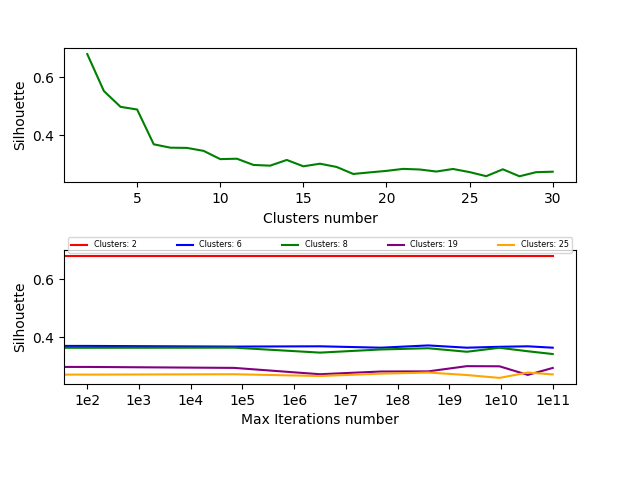
\includegraphics
                [width=\textwidth,keepaspectratio]
                {img/kmeans_chart_Iris_173201.png}
                \caption
                [kmeans chart Iris 173201]{Wykresy wartości Silhouette w zależności od
                zmiennych dla zbioru Iris}
                \label{kmeans_chart_Iris_173201}
            \end{figure}
            \FloatBarrier

%Badania Max Iters dla CUSTOMERS

            \begin{table}[!htbp]
                \begin{minipage}{.48\textwidth}
                    \centering
                    \begin{tabular}{|c|c|}
                        \hline
                        Max iterations & Silhouette \\ \hline
                        1e2 & 0.2931 \\ \hline
                        1e3 & 0.2931 \\ \hline
                        1e4 & 0.2931 \\ \hline
                        1e5 & 0.2931 \\ \hline
                        1e6 & 0.2931 \\ \hline
                        1e7 & 0.2931 \\ \hline
                        1e8 & 0.2931 \\ \hline
                        1e9 & 0.2931 \\ \hline
                        1e10 & 0.2931 \\ \hline
                        1e11 & 0.2931 \\ \hline
                    \end{tabular}
                    \caption
                    [kmeans table iters Customers 2 clusters]{Wartość Silhouette w
                    zależności od liczby maksymalnej iteracji dla liczby klastrów
                    równej 2 dla zbioru Mall Customer Segmentation Data}
                    \label{kmeans_table_iters_Customers_2_clusters}
                \end{minipage}
                \hfill
                \begin{minipage}{.48\textwidth}
                    \centering
                    \begin{tabular}{|c|c|}
                        \hline
                        Max iterations & Silhouette \\ \hline
                        1e2 & 0.4521 \\ \hline
                        1e3 & 0.4521 \\ \hline
                        1e4 & 0.4521 \\ \hline
                        1e5 & 0.4521 \\ \hline
                        1e6 & 0.4521 \\ \hline
                        1e7 & 0.4521 \\ \hline
                        1e8 & 0.4521 \\ \hline
                        1e9 & 0.4521 \\ \hline
                        1e10 & 0.4521 \\ \hline
                        1e11 & 0.4521 \\ \hline
                    \end{tabular}
                    \caption
                    [kmeans table iters Customers 6 clusters]{Wartość Silhouette w
                    zależności od liczby maksymalnej iteracji dla liczby klastrów
                    równej 6 dla zbioru Mall Customer Segmentation Data}
                    \label{kmeans_table_iters_Customers_6_clusters}
                \end{minipage}
                \hfill
            \end{table}
            \FloatBarrier
            \begin{table}[!htbp]
                \begin{minipage}{.48\textwidth}
                    \centering
                    \begin{tabular}{|c|c|}
                        \hline
                        Max iterations & Silhouette \\ \hline
                        1e2 & 0.426 \\ \hline
                        1e3 & 0.4259 \\ \hline
                        1e4 & 0.4259 \\ \hline
                        1e5 & 0.4294 \\ \hline
                        1e6 & 0.4278 \\ \hline
                        1e7 & 0.4259 \\ \hline
                        1e8 & 0.4275 \\ \hline
                        1e9 & 0.4259 \\ \hline
                        1e10 & 0.4295 \\ \hline
                        1e11 & 0.4333 \\ \hline
                    \end{tabular}
                    \caption
                    [kmeans table iters Customers 8 clusters]{Wartość Silhouette w
                    zależności od liczby maksymalnej iteracji dla liczby klastrów
                    równej 8 dla zbioru Mall Customer Segmentation Data}
                    \label{kmeans_table_iters_Customers_8_clusters}
                \end{minipage}
                \hfill
                \begin{minipage}{.48\textwidth}
                    \centering
                    \begin{tabular}{|c|c|}
                        \hline
                        Max iterations & Silhouette \\ \hline
                        1e2 & 0.346 \\ \hline
                        1e3 & 0.33 \\ \hline
                        1e4 & 0.3256 \\ \hline
                        1e5 & 0.3386 \\ \hline
                        1e6 & 0.3279 \\ \hline
                        1e7 & 0.3414 \\ \hline
                        1e8 & 0.3315 \\ \hline
                        1e9 & 0.3429 \\ \hline
                        1e10 & 0.3313 \\ \hline
                        1e11 & 0.3391 \\ \hline
                    \end{tabular}
                    \caption
                    [kmeans table iters Customers 19 clusters]{Wartość Silhouette w
                    zależności od liczby maksymalnej iteracji dla liczby klastrów
                    równej 19 dla zbioru Mall Customer Segmentation Data}
                    \label{kmeans_table_iters_Customers_19_clusters}
                \end{minipage}
                \hfill
            \end{table}
            \FloatBarrier
            \begin{table}[!htbp]
                \begin{minipage}{.5\textwidth}
                    \centering
                    \begin{tabular}{|c|c|}
                        \hline
                        Max iterations & Silhouette \\ \hline
                        1e2 & 0.3388 \\ \hline
                        1e3 & 0.3253 \\ \hline
                        1e4 & 0.3349 \\ \hline
                        1e5 & 0.3395 \\ \hline
                        1e6 & 0.3401 \\ \hline
                        1e7 & 0.32 \\ \hline
                        1e8 & 0.3344 \\ \hline
                        1e9 & 0.3291 \\ \hline
                        1e10 & 0.3428 \\ \hline
                        1e11 & 0.3301 \\ \hline
                    \end{tabular}
                    \caption
                    [kmeans table iters Customers 25 clusters]{Wartość Silhouette w
                    zależności od liczby maksymalnej iteracji dla liczby klastrów
                    równej 25 dla zbioru Mall Customer Segmentation Data}
                    \label{kmeans_table_iters_Customers_25_clusters}
                \end{minipage}
                \hfill
            \end{table}
            \FloatBarrier
            \begin{figure}[!htbp]
                \centering
                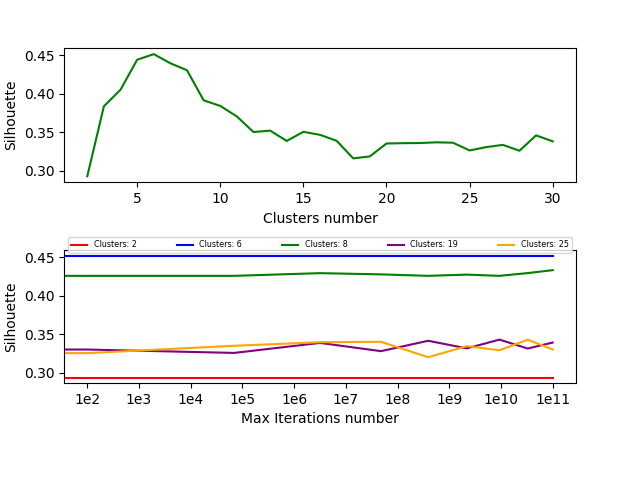
\includegraphics
                [width=\textwidth,keepaspectratio]
                {img/kmeans_chart_Customers_173204.png}
                \caption
                [kmeans chart Customers 173204]{Wykresy wartości Silhouette w
                zależności od zmiennych dla zbioru Mall Customer Segmentation Data}
                \label{kmeans_chart_Customers_173204}
            \end{figure}
            \FloatBarrier

%Badania Max Iters dla MOONS

            \begin{table}[!htbp]
                \begin{minipage}{.48\textwidth}
                    \centering
                    \begin{tabular}{|c|c|}
                        \hline
                        Max iterations & Silhouette \\ \hline
                        1e2 & 0.4907 \\ \hline
                        1e3 & 0.4907 \\ \hline
                        1e4 & 0.4909 \\ \hline
                        1e5 & 0.4907 \\ \hline
                        1e6 & 0.4907 \\ \hline
                        1e7 & 0.4907 \\ \hline
                        1e8 & 0.4907 \\ \hline
                        1e9 & 0.4907 \\ \hline
                        1e10 & 0.4907 \\ \hline
                        1e11 & 0.4907 \\ \hline
                    \end{tabular}
                    \caption
                    [kmeans table iters Moons 2 clusters]{Wartość Silhouette w
                    zależności od liczby maksymalnej iteracji dla liczby klastrów
                    równej 2 dla zbioru Moons}
                    \label{kmeans_table_iters_Moons_2_clusters}
                \end{minipage}
                \hfill
                \begin{minipage}{.48\textwidth}
                    \centering
                    \begin{tabular}{|c|c|}
                        \hline
                        Max iterations & Silhouette \\ \hline
                        1e2 & 0.4945 \\ \hline
                        1e3 & 0.4945 \\ \hline
                        1e4 & 0.4938 \\ \hline
                        1e5 & 0.494 \\ \hline
                        1e6 & 0.4943 \\ \hline
                        1e7 & 0.4945 \\ \hline
                        1e8 & 0.4945 \\ \hline
                        1e9 & 0.4943 \\ \hline
                        1e10 & 0.4936 \\ \hline
                        1e11 & 0.494 \\ \hline
                    \end{tabular}
                    \caption
                    [kmeans table iters Moons 6 clusters]{Wartość Silhouette w
                    zależności od liczby maksymalnej iteracji dla liczby klastrów
                    równej 6 dla zbioru Moons}
                    \label{kmeans_table_iters_Moons_6_clusters}
                \end{minipage}
                \hfill
            \end{table}
            \FloatBarrier
            \begin{table}[!htbp]
                \begin{minipage}{.48\textwidth}
                    \centering
                    \begin{tabular}{|c|c|}
                        \hline
                        Max iterations & Silhouette \\ \hline
                        1e2 & 0.5114 \\ \hline
                        1e3 & 0.5114 \\ \hline
                        1e4 & 0.5113 \\ \hline
                        1e5 & 0.5139 \\ \hline
                        1e6 & 0.5126 \\ \hline
                        1e7 & 0.5114 \\ \hline
                        1e8 & 0.5113 \\ \hline
                        1e9 & 0.5114 \\ \hline
                        1e10 & 0.5114 \\ \hline
                        1e11 & 0.5114 \\ \hline
                    \end{tabular}
                    \caption
                    [kmeans table iters Moons 8 clusters]{Wartość Silhouette w
                    zależności od liczby maksymalnej iteracji dla liczby klastrów
                    równej 8 dla zbioru Moons}
                    \label{kmeans_table_iters_Moons_8_clusters}
                \end{minipage}
                \hfill
                \begin{minipage}{.48\textwidth}
                    \centering
                    \begin{tabular}{|c|c|}
                        \hline
                        Max iterations & Silhouette \\ \hline
                        1e2 & 0.4224 \\ \hline
                        1e3 & 0.4279 \\ \hline
                        1e4 & 0.4212 \\ \hline
                        1e5 & 0.4258 \\ \hline
                        1e6 & 0.4216 \\ \hline
                        1e7 & 0.4197 \\ \hline
                        1e8 & 0.4183 \\ \hline
                        1e9 & 0.4213 \\ \hline
                        1e10 & 0.4241 \\ \hline
                        1e11 & 0.4214 \\ \hline
                    \end{tabular}
                    \caption
                    [kmeans table iters Moons 19 clusters]{Wartość Silhouette w
                    zależności od liczby maksymalnej iteracji dla liczby klastrów
                    równej 19 dla zbioru Moonss}
                    \label{kmeans_table_iters_Moons_19_clusters}
                \end{minipage}
                \hfill
            \end{table}
            \FloatBarrier
            \begin{table}[!htbp]
                \begin{minipage}{.5\textwidth}
                    \centering
                    \begin{tabular}{|c|c|}
                        \hline
                        Max iterations & Silhouette \\ \hline
                        1e2 & 0.3757 \\ \hline
                        1e3 & 0.3757 \\ \hline
                        1e4 & 0.3745 \\ \hline
                        1e5 & 0.3711 \\ \hline
                        1e6 & 0.3813 \\ \hline
                        1e7 & 0.3778 \\ \hline
                        1e8 & 0.3837 \\ \hline
                        1e9 & 0.3913 \\ \hline
                        1e10 & 0.387 \\ \hline
                        1e11 & 0.3833 \\ \hline
                    \end{tabular}
                    \caption
                    [kmeans table iters Moons 25 clusters]{Wartość Silhouette w
                    zależności od liczby maksymalnej iteracji dla liczby klastrów
                    równej 25 dla zbioru Moons}
                    \label{kmeans_table_iters_Moons_25_clusters}
                \end{minipage}
                \hfill
            \end{table}
            \FloatBarrier
            \begin{figure}[!htbp]
                \centering
                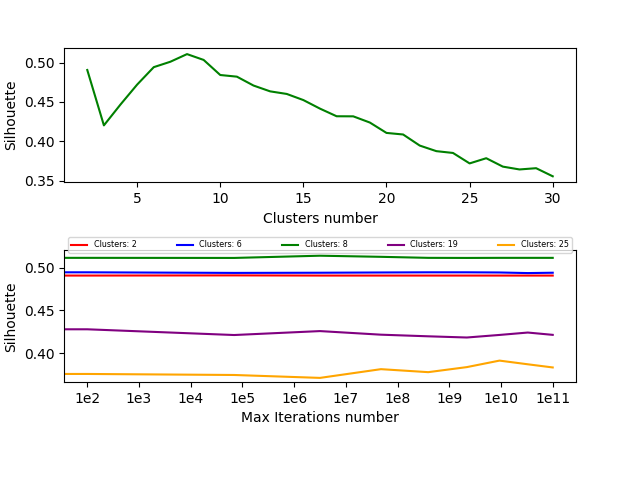
\includegraphics
                [width=\textwidth,keepaspectratio]
                {img/kmeans_chart_Moons_173215.png}
                \caption
                [kmeans chart Moons 173215]{Wykresy wartości Silhouette w zależności od
                zmiennych dla zbioru Moons}
                \label{kmeans_chart_Moons_173215}
            \end{figure}
            \FloatBarrier

        }
        \newpage

        \subsection{Algorytm aglomeracyjny}
        \label{result_2} {
            \begin{figure}[h]
                \centering
                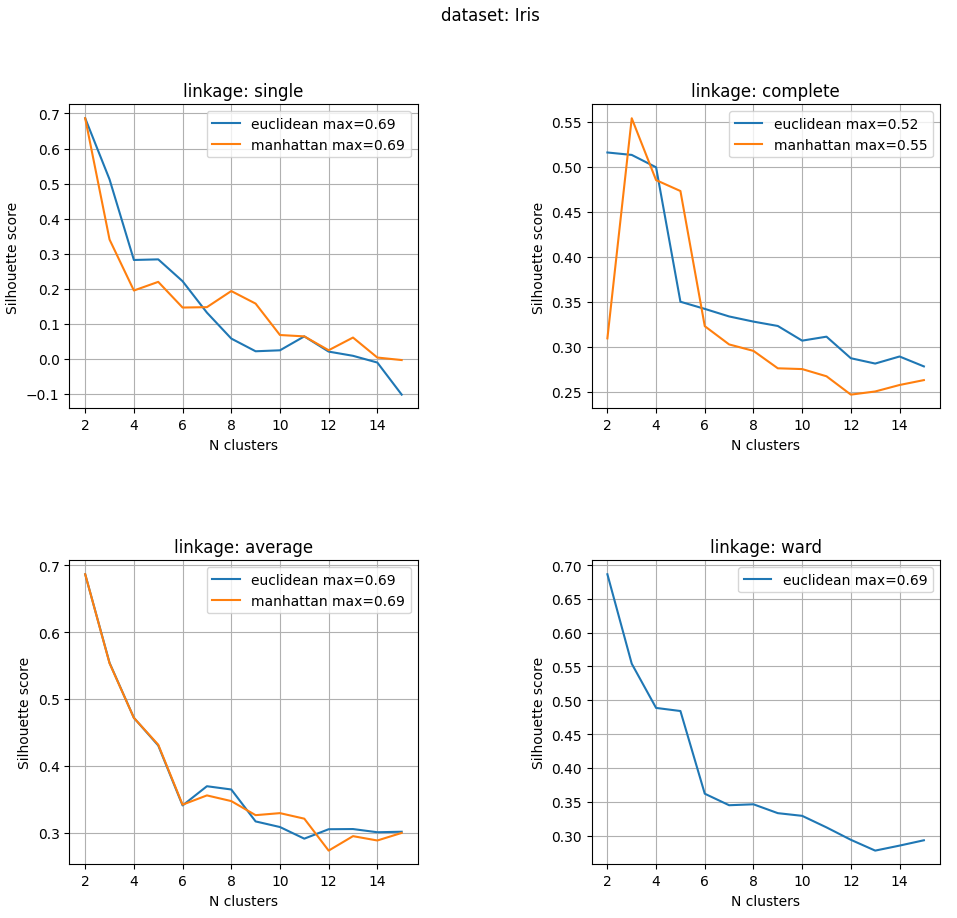
\includegraphics[width=1\textwidth]{img/mum_agglomerative_iris.png}
                \caption{Wyniki działania algorytmu aglomeracyjnego dla zbioru danych ,
                ,Iris Species''}
                \label{fig:agglomerative_iris}
            \end{figure}
            \begin{figure}[h]
                \centering
                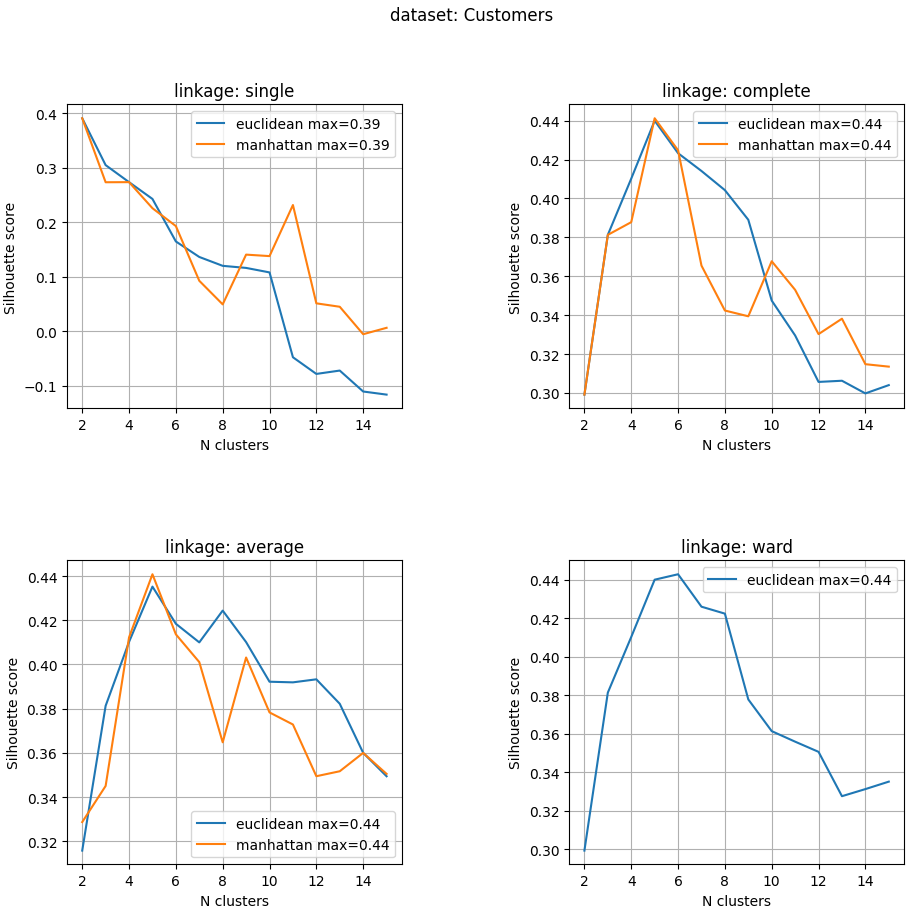
\includegraphics[width=1\textwidth]{img/mum_agglomerative_customers.png}
                \caption{Wyniki działania algorytmu aglomeracyjnego dla zbioru danych ,
                ,Mall Customer Segmentation Data''}
                \label{fig:agglomerative_customers}
            \end{figure}
            \begin{figure}[h]
                \centering
                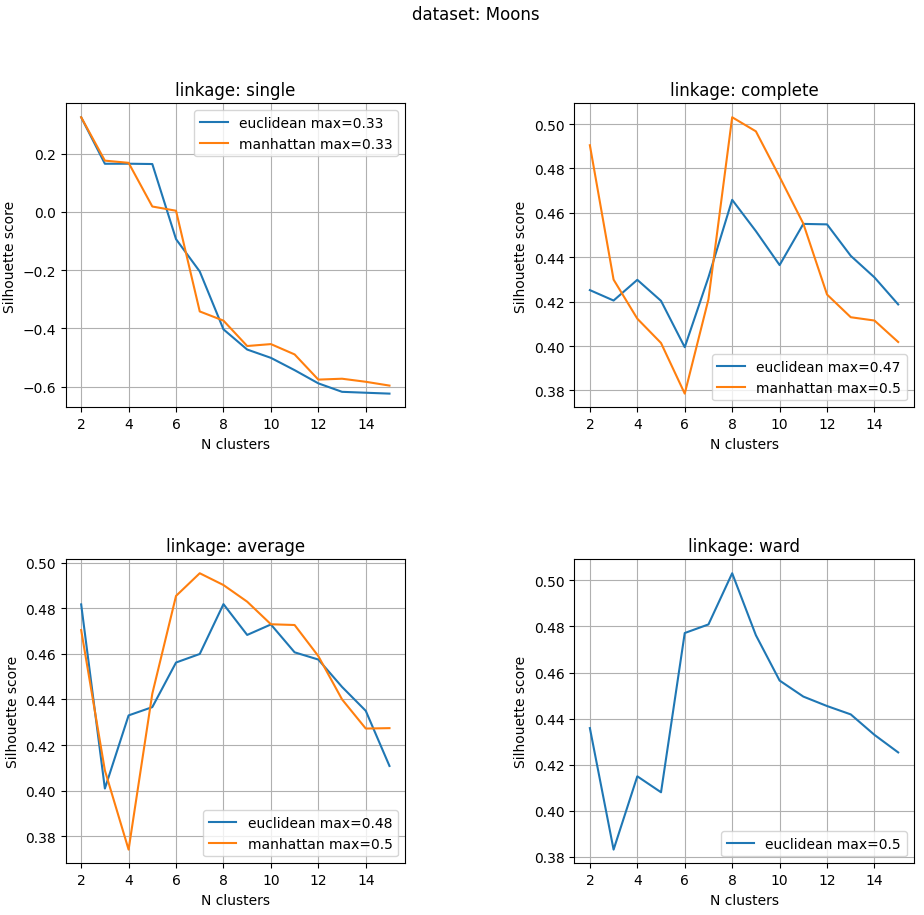
\includegraphics[width=1\textwidth]{img/mum_agglomerative_moons.png}
                \caption{Wyniki działania algorytmu aglomeracyjnego dla zbioru danych ,
                ,Moons''}
                \label{fig:agglomerative_moons}
            \end{figure}
            \FloatBarrier
        }
        \newpage

        \subsection{Algorytm EM}
        \label{result_3} {
            \begin{figure}[!htbp]
            \centering
            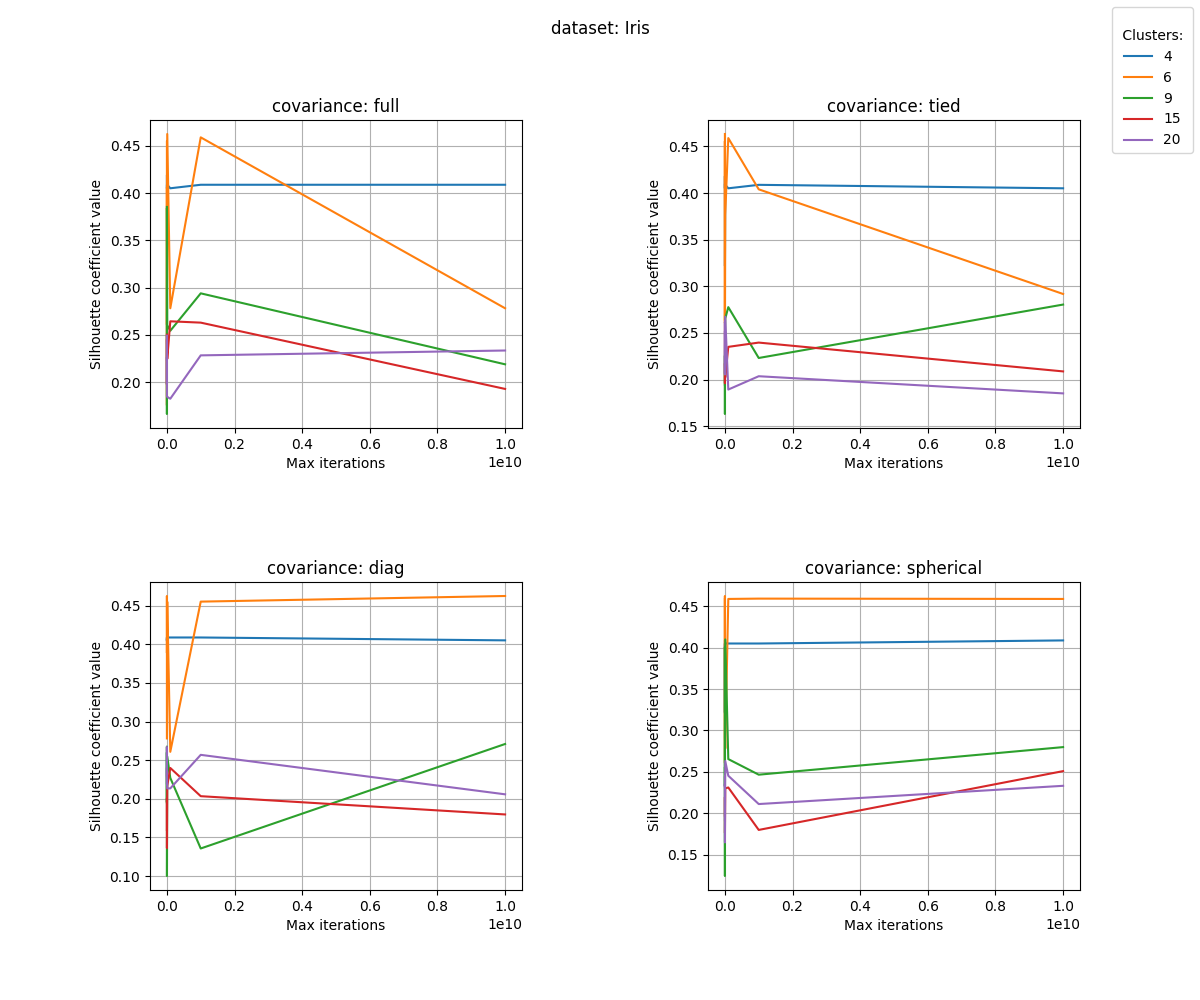
\includegraphics
            [width=\textwidth,keepaspectratio]
            {img/em_scan_chart_Iris-211458.png}
            \caption
            [em scan chart Iris 211458]
            {Wyniki działania algorytmu EM dla zbioru danych Irysów w zależności od
            liczby iteracji i wybranej macierzy kowariancji dla różnej liczby klastrów}
            \label{em_scan_chart_Iris-211458}
            \end{figure}    
        
            \begin{table}[!htbp]
                \begin{minipage}{1\textwidth}
                \centering
                \begin{tabular}{|c|c|c|c|c|}
                \hline
                Max iterations & full & tied & diag & spherical \\ \hline
                40 & 0.405 & 0.409 & 0.409 & 0.405 \\ \hline
                60 & 0.322 & 0.405 & 0.405 & 0.409 \\ \hline
                80 & 0.405 & 0.322 & 0.409 & 0.409 \\ \hline
                100 & 0.409 & 0.405 & 0.409 & 0.322 \\ \hline
                200 & 0.409 & 0.405 & 0.405 & 0.405 \\ \hline
                1000 & 0.409 & 0.405 & 0.405 & 0.376 \\ \hline
                10000 & 0.405 & 0.409 & 0.405 & 0.405 \\ \hline
                100000 & 0.405 & 0.418 & 0.409 & 0.322 \\ \hline
                1000000 & 0.409 & 0.322 & 0.405 & 0.409 \\ \hline
                10000000 & 0.409 & 0.409 & 0.409 & 0.405 \\ \hline
                100000000 & 0.405 & 0.405 & 0.409 & 0.405 \\ \hline
                1000000000 & 0.409 & 0.409 & 0.409 & 0.405 \\ \hline
                10000000000 & 0.409 & 0.405 & 0.405 & 0.409 \\ \hline
                \end{tabular}
                \caption
                [Iris 4 211451]
                {Wartości silhouette dla zbioru danych Irysów w zależności
                od liczby iteracji i wybranej macierzy kowariancji przy 4 klastrach}
                \label{Iris_4_211451}
                \end{minipage}
                \hfill
    
                \begin{minipage}{1\textwidth}
                \centering
                \begin{tabular}{|c|c|c|c|c|}
                \hline
                Max iterations & full & tied & diag & spherical \\ \hline
                40 & 0.278 & 0.278 & 0.261 & 0.406 \\ \hline
                60 & 0.292 & 0.427 & 0.261 & 0.399 \\ \hline
                80 & 0.463 & 0.261 & 0.458 & 0.455 \\ \hline
                100 & 0.459 & 0.377 & 0.263 & 0.459 \\ \hline
                200 & 0.465 & 0.459 & 0.292 & 0.459 \\ \hline
                1000 & 0.28 & 0.261 & 0.292 & 0.261 \\ \hline
                10000 & 0.176 & 0.263 & 0.463 & 0.412 \\ \hline
                100000 & 0.406 & 0.456 & 0.459 & 0.463 \\ \hline
                1000000 & 0.261 & 0.263 & 0.389 & 0.292 \\ \hline
                10000000 & 0.463 & 0.377 & 0.455 & 0.278 \\ \hline
                100000000 & 0.278 & 0.459 & 0.261 & 0.459 \\ \hline
                1000000000 & 0.459 & 0.404 & 0.455 & 0.459 \\ \hline
                10000000000 & 0.278 & 0.292 & 0.463 & 0.459 \\ \hline
                \end{tabular}
                \caption
                [Iris 6 211451]
                {Wartości silhouette dla zbioru danych Irysów w zależności od liczby
                iteracji i wybranej macierzy kowariancji przy 6 klastrach}
                \label{Iris_6_211451}
                \end{minipage}
                \hfill
                
                \centering
                \begin{tabular}{|c|c|c|c|c|}
                \hline
                Max iterations & full & tied & diag & spherical \\ \hline
                40 & 0.241 & 0.394 & 0.243 & 0.246 \\ \hline
                60 & 0.257 & 0.435 & 0.163 & 0.147 \\ \hline
                80 & 0.243 & 0.254 & 0.278 & 0.27 \\ \hline
                100 & 0.216 & 0.248 & 0.248 & 0.229 \\ \hline
                200 & 0.245 & 0.211 & 0.162 & 0.277 \\ \hline
                1000 & 0.244 & 0.203 & 0.26 & 0.124 \\ \hline
                10000 & 0.23 & 0.226 & 0.196 & 0.401 \\ \hline
                100000 & 0.166 & 0.163 & 0.268 & 0.233 \\ \hline
                1000000 & 0.384 & 0.227 & 0.1 & 0.28 \\ \hline
                10000000 & 0.26 & 0.265 & 0.255 & 0.41 \\ \hline
                100000000 & 0.254 & 0.278 & 0.227 & 0.265 \\ \hline
                1000000000 & 0.294 & 0.223 & 0.136 & 0.247 \\ \hline
                10000000000 & 0.219 & 0.28 & 0.271 & 0.28 \\ \hline
                \end{tabular}
                \caption
                [Iris 9 211453]
                {Wartości silhouette dla zbioru danych Irysów w zależności od liczby
                iteracji i wybranej macierzy kowariancji przy 9 klastrach}
                \label{Iris_9_211453}
                \hfill
            
            \end{table}
            
            \begin{table}[!htbp]
                \begin{minipage}{1\textwidth}
                \centering
                \begin{tabular}{|c|c|c|c|c|}
                \hline
                Max iterations & full & tied & diag & spherical \\ \hline
                40 & 0.202 & 0.182 & 0.159 & 0.247 \\ \hline
                60 & 0.246 & 0.173 & 0.196 & 0.241 \\ \hline
                80 & 0.168 & 0.175 & 0.227 & 0.227 \\ \hline
                100 & 0.197 & 0.233 & 0.202 & 0.18 \\ \hline
                200 & 0.236 & 0.138 & 0.147 & 0.24 \\ \hline
                1000 & 0.243 & 0.218 & 0.201 & 0.212 \\ \hline
                10000 & 0.198 & 0.203 & 0.19 & 0.218 \\ \hline
                100000 & 0.211 & 0.196 & 0.155 & 0.219 \\ \hline
                1000000 & 0.245 & 0.217 & 0.136 & 0.176 \\ \hline
                10000000 & 0.225 & 0.202 & 0.217 & 0.23 \\ \hline
                100000000 & 0.264 & 0.235 & 0.24 & 0.231 \\ \hline
                1000000000 & 0.263 & 0.24 & 0.203 & 0.18 \\ \hline
                10000000000 & 0.193 & 0.209 & 0.18 & 0.251 \\ \hline
                \end{tabular}
                \caption
                [Iris 15 211456]
                {Wartości silhouette dla zbioru danych Irysów w zależności od liczby
                iteracji i wybranej macierzy kowariancji przy 15 klastrach}
                \label{Iris_15_211456}
                \end{minipage}
                \hfill            
            
                \begin{minipage}{1\textwidth}
                \centering
                \begin{tabular}{|c|c|c|c|c|}
                \hline
                Max iterations & full & tied & diag & spherical \\ \hline
                40 & 0.204 & 0.227 & 0.232 & 0.235 \\ \hline
                60 & 0.219 & 0.261 & 0.231 & 0.095 \\ \hline
                80 & 0.239 & 0.238 & 0.253 & 0.232 \\ \hline
                100 & 0.182 & 0.26 & 0.222 & 0.194 \\ \hline
                200 & 0.195 & 0.238 & 0.187 & 0.227 \\ \hline
                1000 & 0.226 & 0.25 & 0.24 & 0.235 \\ \hline
                10000 & 0.198 & 0.206 & 0.219 & 0.231 \\ \hline
                100000 & 0.249 & 0.262 & 0.267 & 0.244 \\ \hline
                1000000 & 0.185 & 0.205 & 0.228 & 0.165 \\ \hline
                10000000 & 0.184 & 0.267 & 0.213 & 0.263 \\ \hline
                100000000 & 0.182 & 0.189 & 0.213 & 0.245 \\ \hline
                1000000000 & 0.228 & 0.204 & 0.257 & 0.211 \\ \hline
                10000000000 & 0.233 & 0.185 & 0.206 & 0.233 \\ \hline
                \end{tabular}
                \caption
                [Iris 20 211458]
                {Wartości silhouette dla zbioru danych Irysów w zależności od liczby
                iteracji i wybranej macierzy kowariancji przy 20 klastrach}
                \label{Iris_20_211458}
                \end{minipage}
                \hfill
            \end{table}
            
            \begin{figure}[!htbp]
            \centering
            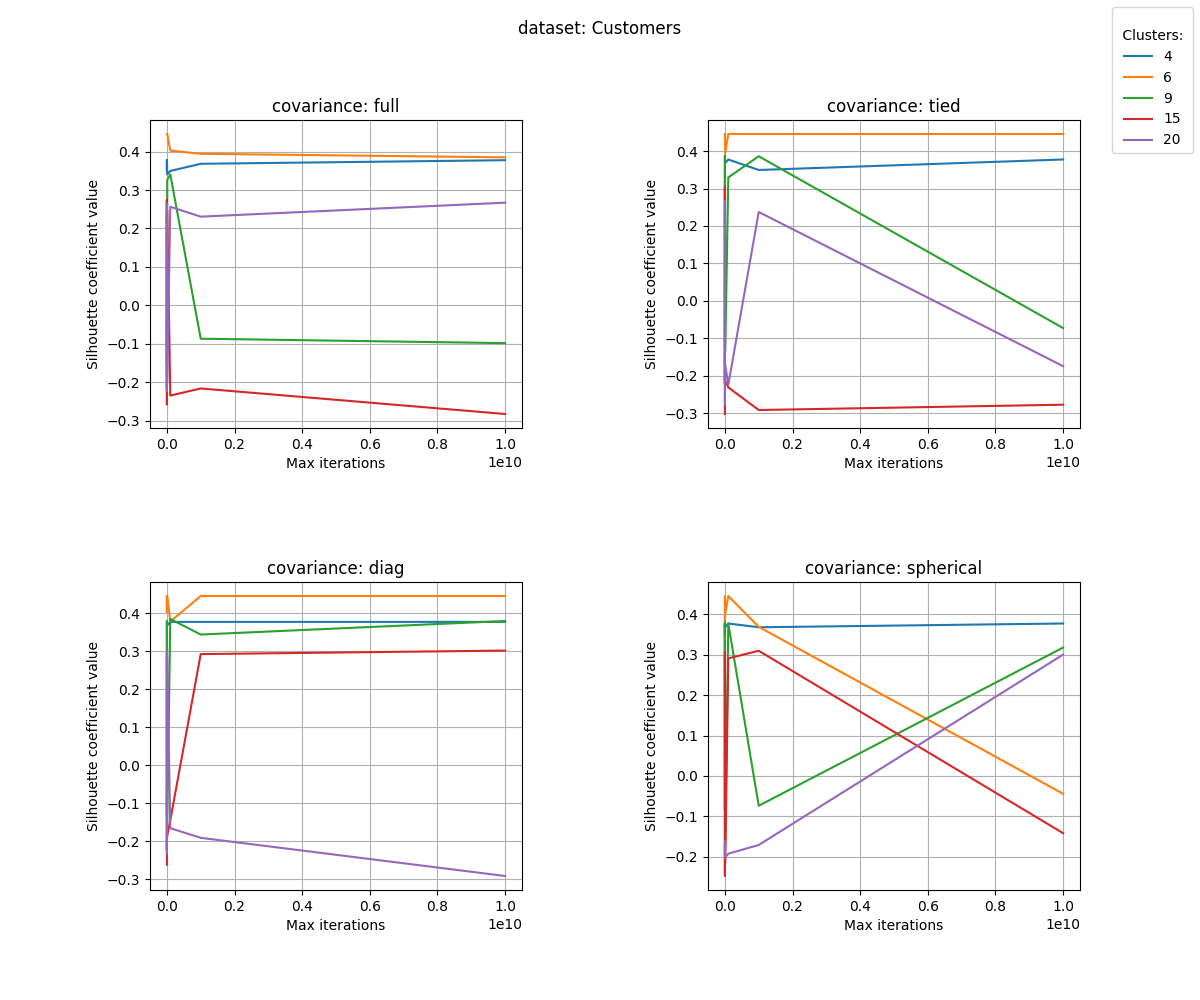
\includegraphics
            [width=\textwidth,keepaspectratio]
            {img/em_scan_chart_Customers-211509.png}
            \caption
            [em scan chart Customers 211509]
            {Wyniki działania algorytmu EM dla zbioru danych Customers w zależności
            od liczby iteracji i wybranej macierzy kowariancji dla różnej liczby klastrów}
            \label{em_scan_chart_Customers-211509}
            \end{figure}
            
            \begin{table}[!htbp]
                \begin{minipage}{1\textwidth}
                \centering
                \begin{tabular}{|c|c|c|c|c|}
                \hline
                Max iterations & full & tied & diag & spherical \\ \hline
                40 & 0.368 & 0.377 & 0.377 & 0.377 \\ \hline
                60 & 0.377 & 0.377 & 0.377 & 0.377 \\ \hline
                80 & 0.377 & 0.368 & 0.377 & 0.377 \\ \hline
                100 & 0.377 & 0.377 & 0.377 & 0.377 \\ \hline
                200 & 0.377 & 0.368 & 0.377 & 0.377 \\ \hline
                1000 & 0.349 & 0.377 & 0.377 & 0.377 \\ \hline
                10000 & 0.377 & 0.377 & 0.377 & 0.349 \\ \hline
                100000 & 0.377 & 0.377 & 0.377 & 0.377 \\ \hline
                1000000 & 0.377 & 0.368 & 0.377 & 0.368 \\ \hline
                10000000 & 0.34 & 0.368 & 0.368 & 0.368 \\ \hline
                100000000 & 0.349 & 0.377 & 0.377 & 0.377 \\ \hline
                1000000000 & 0.368 & 0.349 & 0.377 & 0.368 \\ \hline
                10000000000 & 0.377 & 0.377 & 0.377 & 0.377 \\ \hline
                \end{tabular}
                \caption
                [Customers 4 211459]
                {Wartości silhouette dla zbioru danych Customers w zależności od liczby
                iteracji i wybranej macierzy kowariancji przy 4 klastrach}
                \label{Customers_4_211459}
                \end{minipage}
                \hfill
                
                \begin{minipage}{1\textwidth}
                \centering
                \begin{tabular}{|c|c|c|c|c|}
                \hline
                Max iterations & full & tied & diag & spherical \\ \hline
                40 & 0.371 & 0.446 & 0.446 & -0.006 \\ \hline
                60 & 0.446 & 0.394 & 0.383 & 0.394 \\ \hline
                80 & 0.394 & 0.001 & 0.446 & 0.446 \\ \hline
                100 & 0.406 & 0.446 & 0.446 & 0.402 \\ \hline
                200 & 0.385 & 0.446 & 0.446 & 0.446 \\ \hline
                1000 & 0.446 & 0.446 & 0.446 & 0.446 \\ \hline
                10000 & 0.446 & 0.446 & 0.403 & 0.446 \\ \hline
                100000 & 0.446 & 0.446 & 0.446 & 0.446 \\ \hline
                1000000 & 0.446 & 0.446 & 0.446 & 0.446 \\ \hline
                10000000 & 0.446 & 0.394 & 0.446 & 0.402 \\ \hline
                100000000 & 0.402 & 0.446 & 0.378 & 0.446 \\ \hline
                1000000000 & 0.394 & 0.446 & 0.446 & 0.369 \\ \hline
                10000000000 & 0.385 & 0.446 & 0.446 & -0.044 \\ \hline
                \end{tabular}
                \caption
                [Customers 6 211500]
                {Wartości silhouette dla zbioru danych Customers w zależności od liczby
                iteracji i wybranej macierzy kowariancji przy 6 klastrach}
                \label{Customers_6_211500}
                \end{minipage}
                \hfill

                \begin{minipage}{1\textwidth}
                \centering
                \begin{tabular}{|c|c|c|c|c|}
                \hline
                Max iterations & full & tied & diag & spherical \\ \hline
                40 & -0.073 & 0.363 & 0.387 & 0.28 \\ \hline
                60 & -0.137 & -0.086 & -0.086 & 0.379 \\ \hline
                80 & -0.136 & -0.232 & -0.133 & 0.346 \\ \hline
                100 & -0.074 & 0.353 & 0.361 & 0.292 \\ \hline
                200 & 0.354 & -0.299 & -0.074 & -0.112 \\ \hline
                1000 & 0.273 & 0.349 & -0.094 & -0.085 \\ \hline
                10000 & -0.153 & -0.22 & -0.133 & 0.374 \\ \hline
                100000 & -0.113 & -0.071 & 0.305 & 0.328 \\ \hline
                1000000 & -0.086 & 0.388 & 0.38 & 0.294 \\ \hline
                10000000 & 0.326 & -0.135 & -0.156 & -0.17 \\ \hline
                100000000 & 0.34 & 0.33 & 0.385 & 0.377 \\ \hline
                1000000000 & -0.086 & 0.386 & 0.344 & -0.074 \\ \hline
                10000000000 & -0.098 & -0.073 & 0.38 & 0.318 \\ \hline
                \end{tabular}
                \caption
                [Customers 9 211503]
                {Wartości silhouette dla zbioru danych Customers w zależności od liczby
                iteracji i wybranej macierzy kowariancji przy 9 klastrach}
                \label{Customers_9_211503}
                \end{minipage}
                \hfill
            
            \end{table}
            
            \begin{table}[!htbp]
                \begin{minipage}{1\textwidth}
                \centering
                \begin{tabular}{|c|c|c|c|c|}
                \hline
                Max iterations & full & tied & diag & spherical \\ \hline
                40 & 0.327 & 0.273 & 0.319 & 0.27 \\ \hline
                60 & -0.167 & -0.204 & 0.281 & 0.303 \\ \hline
                80 & -0.275 & -0.181 & 0.291 & -0.246 \\ \hline
                100 & 0.326 & -0.198 & 0.292 & 0.258 \\ \hline
                200 & 0.247 & 0.301 & -0.274 & -0.292 \\ \hline
                1000 & -0.257 & 0.304 & 0.283 & 0.302 \\ \hline
                10000 & -0.163 & 0.299 & 0.29 & -0.248 \\ \hline
                100000 & 0.275 & -0.21 & -0.221 & -0.197 \\ \hline
                1000000 & -0.216 & -0.206 & -0.195 & 0.299 \\ \hline
                10000000 & 0.248 & -0.214 & -0.185 & -0.215 \\ \hline
                100000000 & -0.234 & -0.231 & -0.144 & 0.291 \\ \hline
                1000000000 & -0.216 & -0.291 & 0.293 & 0.31 \\ \hline
                10000000000 & -0.282 & -0.277 & 0.302 & -0.142 \\ \hline
                \end{tabular}
                \caption
                [Customers 15 211505]
                {Wartości silhouette dla zbioru danych Customers w zależności od
                liczby iteracji i wybranej macierzy kowariancji przy 15 klastrach}
                \label{Customers_15_211505}
                \end{minipage}
                \hfill

                \begin{minipage}{1\textwidth}
                \centering
                \begin{tabular}{|c|c|c|c|c|}
                \hline
                Max iterations & full & tied & diag & spherical \\ \hline
                40 & -0.13 & -0.187 & -0.223 & -0.212 \\ \hline
                60 & -0.259 & -0.2 & -0.225 & -0.167 \\ \hline
                80 & -0.235 & -0.202 & -0.151 & -0.22 \\ \hline
                100 & 0.295 & -0.227 & 0.301 & 0.314 \\ \hline
                200 & 0.279 & -0.202 & 0.285 & -0.254 \\ \hline
                1000 & -0.186 & -0.184 & -0.232 & -0.182 \\ \hline
                10000 & 0.265 & 0.267 & -0.18 & -0.165 \\ \hline
                100000 & -0.223 & -0.214 & 0.256 & -0.161 \\ \hline
                1000000 & 0.239 & -0.223 & 0.297 & -0.198 \\ \hline
                10000000 & -0.202 & -0.171 & 0.281 & -0.201 \\ \hline
                100000000 & 0.256 & -0.224 & -0.165 & -0.192 \\ \hline
                1000000000 & 0.231 & 0.237 & -0.191 & -0.171 \\ \hline
                10000000000 & 0.267 & -0.174 & -0.291 & 0.3 \\ \hline
                \end{tabular}
                \caption
                [Customers 20 211509]
                {Wartości silhouette dla zbioru danych Customers w zależności od
                liczby iteracji i wybranej macierzy kowariancji przy 20 klastrach}
                \label{Customers_20_211509}
                \end{minipage}
                \hfill
            \end{table}
            
            \begin{figure}[!htbp]
            \centering
            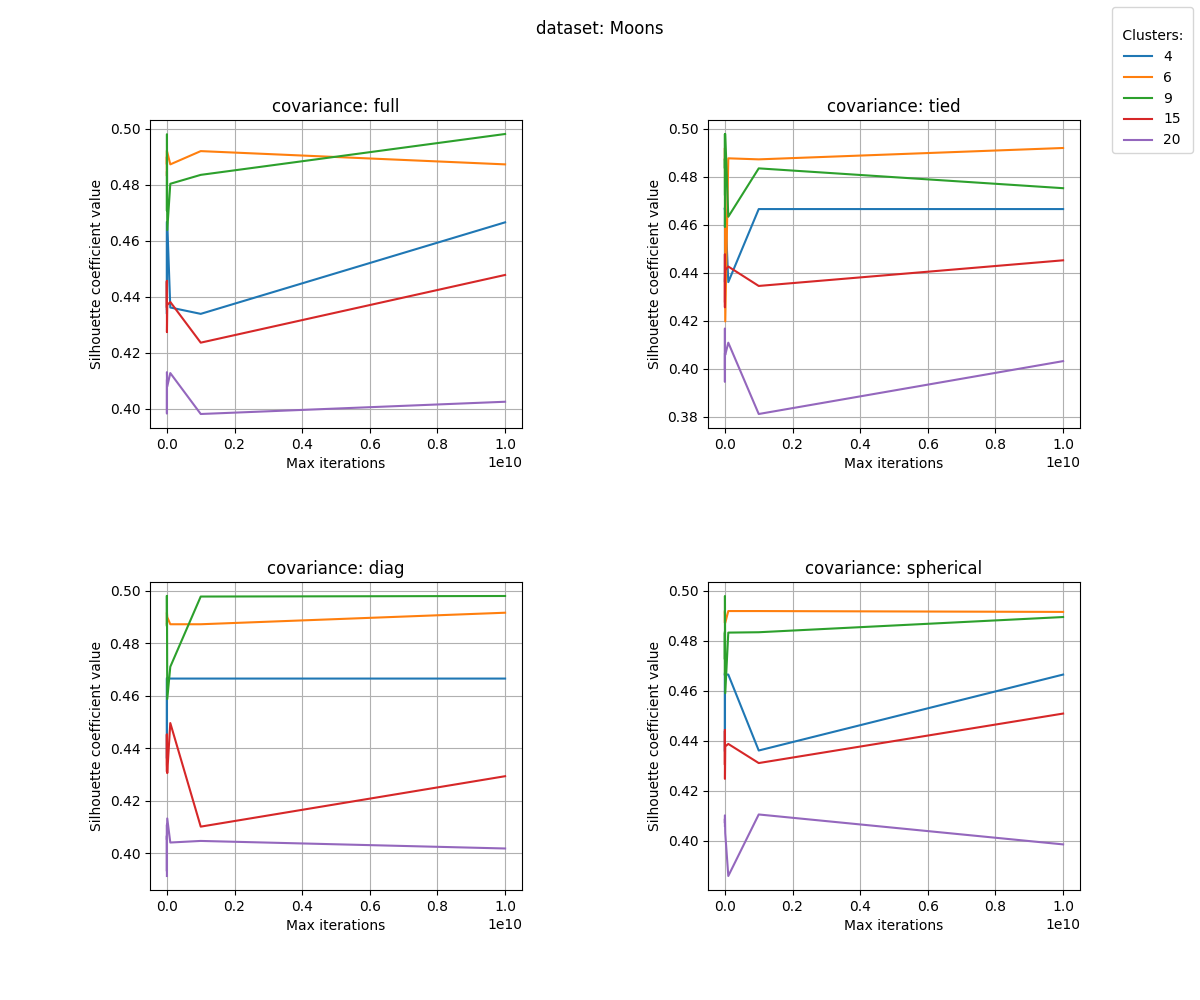
\includegraphics
            [width=\textwidth,keepaspectratio]
            {img/em_scan_chart_Moons-211518.png}
            \caption
            [em scan chart Moons 211518]
            {Wyniki działania algorytmu EM dla zbioru danych Moons w zależności od
            liczby iteracji i wybranej macierzy kowariancji dla różnej liczby klastrów}
            \label{em_scan_chart_Moons-211518}
            \end{figure}
            
            \begin{table}[]
                \begin{minipage}{1\textwidth}
                \centering
                \begin{tabular}{|c|c|c|c|c|}
                \hline
                Max iterations & full & tied & diag & spherical \\ \hline
                40 & 0.467 & 0.436 & 0.436 & 0.467 \\ \hline
                60 & 0.467 & 0.436 & 0.467 & 0.467 \\ \hline
                80 & 0.467 & 0.467 & 0.436 & 0.467 \\ \hline
                100 & 0.467 & 0.467 & 0.467 & 0.434 \\ \hline
                200 & 0.467 & 0.467 & 0.467 & 0.467 \\ \hline
                1000 & 0.434 & 0.467 & 0.436 & 0.467 \\ \hline
                10000 & 0.436 & 0.467 & 0.467 & 0.467 \\ \hline
                100000 & 0.436 & 0.467 & 0.467 & 0.436 \\ \hline
                1000000 & 0.467 & 0.436 & 0.467 & 0.467 \\ \hline
                10000000 & 0.467 & 0.467 & 0.467 & 0.467 \\ \hline
                100000000 & 0.436 & 0.436 & 0.467 & 0.467 \\ \hline
                1000000000 & 0.434 & 0.467 & 0.467 & 0.436 \\ \hline
                10000000000 & 0.467 & 0.467 & 0.467 & 0.467 \\ \hline
                \end{tabular}
                \caption
                [Moons 4 211511]{Wartości silhouette dla zbioru danych Moons w
                zależności od liczby iteracji i wybranej macierzy kowariancji przy 4
                klastrach}
                \label{Moons_4_211511}
                \end{minipage}
                \hfill

                \begin{minipage}{1\textwidth}
                \centering
                \begin{tabular}{|c|c|c|c|c|}
                \hline
                Max iterations & full & tied & diag & spherical \\ \hline
                40 & 0.488 & 0.492 & 0.492 & 0.409 \\ \hline
                60 & 0.492 & 0.492 & 0.487 & 0.487 \\ \hline
                80 & 0.488 & 0.487 & 0.487 & 0.492 \\ \hline
                100 & 0.492 & 0.492 & 0.492 & 0.487 \\ \hline
                200 & 0.492 & 0.492 & 0.487 & 0.492 \\ \hline
                1000 & 0.483 & 0.492 & 0.487 & 0.492 \\ \hline
                10000 & 0.49 & 0.492 & 0.492 & 0.487 \\ \hline
                100000 & 0.487 & 0.487 & 0.492 & 0.487 \\ \hline
                1000000 & 0.492 & 0.488 & 0.492 & 0.492 \\ \hline
                10000000 & 0.492 & 0.42 & 0.49 & 0.487 \\ \hline
                100000000 & 0.487 & 0.488 & 0.487 & 0.492 \\ \hline
                1000000000 & 0.492 & 0.487 & 0.487 & 0.492 \\ \hline
                10000000000 & 0.487 & 0.492 & 0.492 & 0.492 \\ \hline
                \end{tabular}
                \caption
                [Moons 6 211512]{Wartości silhouette dla zbioru danych Moons w
                zależności od liczby iteracji i wybranej macierzy kowariancji przy 6
                klastrach}
                \label{Moons_6_211512}
                \end{minipage}
                \hfill
                
                \begin{minipage}{1\textwidth}
                \centering
                \begin{tabular}{|c|c|c|c|c|}
                \hline
                Max iterations & full & tied & diag & spherical \\ \hline
                40 & 0.463 & 0.498 & 0.487 & 0.49 \\ \hline
                60 & 0.463 & 0.488 & 0.498 & 0.498 \\ \hline
                80 & 0.498 & 0.473 & 0.459 & 0.498 \\ \hline
                100 & 0.498 & 0.481 & 0.498 & 0.498 \\ \hline
                200 & 0.498 & 0.458 & 0.471 & 0.486 \\ \hline
                1000 & 0.483 & 0.487 & 0.498 & 0.473 \\ \hline
                10000 & 0.471 & 0.483 & 0.486 & 0.483 \\ \hline
                100000 & 0.471 & 0.498 & 0.498 & 0.466 \\ \hline
                1000000 & 0.498 & 0.459 & 0.498 & 0.498 \\ \hline
                10000000 & 0.464 & 0.498 & 0.459 & 0.459 \\ \hline
                100000000 & 0.48 & 0.463 & 0.471 & 0.483 \\ \hline
                1000000000 & 0.483 & 0.483 & 0.498 & 0.483 \\ \hline
                10000000000 & 0.498 & 0.475 & 0.498 & 0.49 \\ \hline
                \end{tabular}
                \caption
                [Moons 9 211514]{Wartości silhouette dla zbioru danych Moons w
                zależności od liczby iteracji i wybranej macierzy kowariancji przy 9
                klastrach}
                \label{Moons_9_211514}
                \end{minipage}
                \hfill

            \end{table}
            
            \begin{table}[!htbp]
                \begin{minipage}{1\textwidth}
                \centering
                \begin{tabular}{|c|c|c|c|c|}
                \hline
                Max iterations & full & tied & diag & spherical \\ \hline
                40 & 0.423 & 0.44 & 0.448 & 0.435 \\ \hline
                60 & 0.451 & 0.451 & 0.422 & 0.434 \\ \hline
                80 & 0.446 & 0.436 & 0.438 & 0.423 \\ \hline
                100 & 0.443 & 0.448 & 0.433 & 0.439 \\ \hline
                200 & 0.44 & 0.421 & 0.42 & 0.436 \\ \hline
                1000 & 0.445 & 0.448 & 0.435 & 0.43 \\ \hline
                10000 & 0.436 & 0.446 & 0.431 & 0.444 \\ \hline
                100000 & 0.446 & 0.426 & 0.445 & 0.429 \\ \hline
                1000000 & 0.427 & 0.437 & 0.434 & 0.425 \\ \hline
                10000000 & 0.437 & 0.441 & 0.431 & 0.438 \\ \hline
                100000000 & 0.438 & 0.443 & 0.45 & 0.439 \\ \hline
                1000000000 & 0.424 & 0.435 & 0.41 & 0.431 \\ \hline
                10000000000 & 0.448 & 0.445 & 0.429 & 0.451 \\ \hline
                \end{tabular}
                \caption
                [Moons 15 211516]{Wartości silhouette dla zbioru danych Moons w
                zależności od liczby iteracji i wybranej macierzy kowariancji przy 15
                klastrach}
                \label{Moons_15_211516}
                \end{minipage}
                \hfill            
            
                \begin{minipage}{1\textwidth}
                \centering
                \begin{tabular}{|c|c|c|c|c|}
                \hline
                Max iterations & full & tied & diag & spherical \\ \hline
                40 & 0.415 & 0.391 & 0.401 & 0.396 \\ \hline
                60 & 0.41 & 0.384 & 0.411 & 0.41 \\ \hline
                80 & 0.394 & 0.412 & 0.391 & 0.395 \\ \hline
                100 & 0.396 & 0.389 & 0.393 & 0.412 \\ \hline
                200 & 0.397 & 0.413 & 0.403 & 0.404 \\ \hline
                1000 & 0.4 & 0.417 & 0.407 & 0.409 \\ \hline
                10000 & 0.398 & 0.395 & 0.393 & 0.409 \\ \hline
                100000 & 0.402 & 0.401 & 0.411 & 0.407 \\ \hline
                1000000 & 0.413 & 0.406 & 0.405 & 0.41 \\ \hline
                10000000 & 0.408 & 0.406 & 0.413 & 0.403 \\ \hline
                100000000 & 0.413 & 0.411 & 0.404 & 0.386 \\ \hline
                1000000000 & 0.398 & 0.381 & 0.405 & 0.411 \\ \hline
                10000000000 & 0.402 & 0.403 & 0.402 & 0.399 \\ \hline
                \end{tabular}
                \caption
                [Moons 20 211518]{Wartości silhouette dla zbioru danych Moons w
                zależności od liczby iteracji i wybranej macierzy kowariancji przy 20
                klastrach}
                \label{Moons_20_211518}
                \end{minipage}
                \hfill
            \end{table}
        }
        \newpage

        \subsection{Algorytm DBSCAN}
        \label{result_4} {

            \subsubsection{Metryka Euklidesowa}
            \label{dbscan_eucl} {

                \begin{table}[!htbp]
                    \begin{minipage}{.24\textwidth}
                        \centering
                        \begin{tabular}{|c|c|}
                            \hline
                            Eps & Silh \\ \hline
                            0.1 & -0.5147 \\ \hline
                            0.2 & -0.2479 \\ \hline
                            0.3 & -0.0026 \\ \hline
                            0.4 & 0.2419 \\ \hline
                            0.5 & 0.1904 \\ \hline
                            0.6 & 0.3646 \\ \hline
                            0.7 & 0.2818 \\ \hline
                            0.8 & 0.5118 \\ \hline
                            0.9 & 0.6864 \\ \hline
                            1.0 & 0.6864 \\ \hline
                            1.1 & 0.6864 \\ \hline
                            1.2 & 0.6864 \\ \hline
                            1.3 & 0.6864 \\ \hline
                            1.4 & 0.6864 \\ \hline
                            1.5 & 0.6864 \\ \hline
                            1.6 & 0.6864 \\ \hline
                        \end{tabular}
                        \caption
                        [Iris, min samples: 2]
                        {Iris, min samples: 2}
                        \label{db_scan_table_Iris_eucl_min_sample2}
                    \end{minipage}
                    \hfill
                    \begin{minipage}{.24\textwidth}
                        \centering
                        \begin{tabular}{|c|c|}
                            \hline
                            Eps & Silh \\ \hline
                            0.1 & 0.0439 \\ \hline
                            0.2 & -0.3396 \\ \hline
                            0.3 & 0.0319 \\ \hline
                            0.4 & 0.3346 \\ \hline
                            0.5 & 0.3463 \\ \hline
                            0.6 & 0.4226 \\ \hline
                            0.7 & 0.5016 \\ \hline
                            0.8 & 0.5118 \\ \hline
                            0.9 & 0.6864 \\ \hline
                            1.0 & 0.6864 \\ \hline
                            1.1 & 0.6864 \\ \hline
                            1.2 & 0.6864 \\ \hline
                            1.3 & 0.6864 \\ \hline
                            1.4 & 0.6864 \\ \hline
                            1.5 & 0.6864 \\ \hline
                            1.6 & 0.6864 \\ \hline
                        \end{tabular}
                        \caption
                        [Iris, min samples: 3]
                        {Iris, min samples: 3}
                        \label{db_scan_table_Iris_eucl_min_sample3}
                    \end{minipage}
                    \hfill
                    \begin{minipage}{.24\textwidth}
                        \centering
                        \begin{tabular}{|c|c|}
                            \hline
                            Eps & Silh \\ \hline
                            0.2 & -0.3275 \\ \hline
                            0.3 & -0.0463 \\ \hline
                            0.4 & 0.3249 \\ \hline
                            0.5 & 0.3809 \\ \hline
                            0.6 & 0.4226 \\ \hline
                            0.7 & 0.5016 \\ \hline
                            0.8 & 0.5118 \\ \hline
                            0.9 & 0.6864 \\ \hline
                            1.0 & 0.6864 \\ \hline
                            1.1 & 0.6864 \\ \hline
                            1.2 & 0.6864 \\ \hline
                            1.3 & 0.6864 \\ \hline
                            1.4 & 0.6864 \\ \hline
                            1.5 & 0.6864 \\ \hline
                            1.6 & 0.6864 \\ \hline
                        \end{tabular}
                        \caption
                        [Iris, min samples: 4]
                        {Iris, min samples: 4}
                        \label{db_scan_table_Iris_eucl_min_sample4}
                    \end{minipage}
                    \hfill
                    \begin{minipage}{.24\textwidth}
                        \centering
                        \begin{tabular}{|c|c|}
                            \hline
                            Eps & Silh \\ \hline
                            0.2 & 0.1945 \\ \hline
                            0.3 & -0.0518 \\ \hline
                            0.4 & 0.2778 \\ \hline
                            0.5 & 0.4858 \\ \hline
                            0.6 & 0.5379 \\ \hline
                            0.7 & 0.5016 \\ \hline
                            0.8 & 0.5118 \\ \hline
                            0.9 & 0.6864 \\ \hline
                            1.0 & 0.6864 \\ \hline
                            1.1 & 0.6864 \\ \hline
                            1.2 & 0.6864 \\ \hline
                            1.3 & 0.6864 \\ \hline
                            1.4 & 0.6864 \\ \hline
                            1.5 & 0.6864 \\ \hline
                            1.6 & 0.6864 \\ \hline
                        \end{tabular}
                        \caption
                        [Iris, min samples: 5]
                        {Iris, min samples: 5}
                        \label{db_scan_table_Iris_eucl_min_sample5}
                    \end{minipage}
                \end{table}
                \FloatBarrier

                \begin{figure}[!htbp]
                    \centering
                    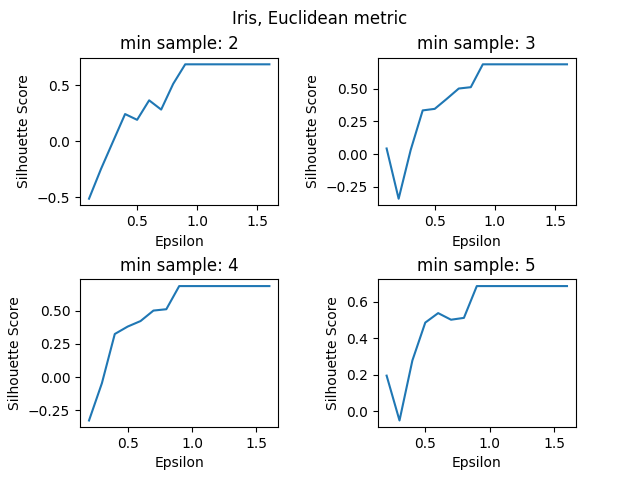
\includegraphics
                    [width=0.95\textwidth,keepaspectratio]
                    {img/db_scan_chart_Iris_eucl0-141824.png}
                    \caption{}
                    \label{db_scan_chart_Iris_eucl0-141824}
                \end{figure}
                \FloatBarrier

                \begin{table}[!htbp]
                    \begin{minipage}{.24\textwidth}
                        \centering
                        \begin{tabular}{|c|c|}
                            \hline
                            Eps & Silh \\ \hline
                            0.2 & 0.1852 \\ \hline
                            0.3 & 0.0408 \\ \hline
                            0.4 & 0.2778 \\ \hline
                            0.5 & 0.477 \\ \hline
                            0.6 & 0.5454 \\ \hline
                            0.7 & 0.5251 \\ \hline
                            0.8 & 0.5118 \\ \hline
                            0.9 & 0.6864 \\ \hline
                            1.0 & 0.6864 \\ \hline
                            1.1 & 0.6864 \\ \hline
                            1.2 & 0.6864 \\ \hline
                            1.3 & 0.6864 \\ \hline
                            1.4 & 0.6864 \\ \hline
                            1.5 & 0.6864 \\ \hline
                            1.6 & 0.6864 \\ \hline
                        \end{tabular}
                        \caption
                        [Iris, min samples: 6]
                        {Iris, min samples: 6}
                        \label{db_scan_table_Iris_eucl_min_sample6}
                    \end{minipage}
                    \hfill
                    \begin{minipage}{.24\textwidth}
                        \centering
                        \begin{tabular}{|c|c|}
                            \hline
                            Eps & Silh \\ \hline
                            0.2 & 0.1734 \\ \hline
                            0.3 & 0.0085 \\ \hline
                            0.4 & 0.1992 \\ \hline
                            0.5 & 0.4641 \\ \hline
                            0.6 & 0.5419 \\ \hline
                            0.7 & 0.5346 \\ \hline
                            0.8 & 0.522 \\ \hline
                            0.9 & 0.6864 \\ \hline
                            1.0 & 0.6864 \\ \hline
                            1.1 & 0.6864 \\ \hline
                            1.2 & 0.6864 \\ \hline
                            1.3 & 0.6864 \\ \hline
                            1.4 & 0.6864 \\ \hline
                            1.5 & 0.6864 \\ \hline
                            1.6 & 0.6864 \\ \hline
                        \end{tabular}
                        \caption
                        [Iris, min samples: 7]
                        {Iris, min samples: 7}
                        \label{db_scan_table_Iris_eucl_min_sample7}
                    \end{minipage}
                    \hfill
                    \begin{minipage}{.24\textwidth}
                        \centering
                        \begin{tabular}{|c|c|}
                            \hline
                            Eps & Silh \\ \hline
                            0.2 & 0.1092 \\ \hline
                            0.3 & 0.4396 \\ \hline
                            0.4 & 0.17 \\ \hline
                            0.5 & 0.4502 \\ \hline
                            0.6 & 0.5419 \\ \hline
                            0.7 & 0.5346 \\ \hline
                            0.8 & 0.522 \\ \hline
                            0.9 & 0.6864 \\ \hline
                            1.0 & 0.6864 \\ \hline
                            1.1 & 0.6864 \\ \hline
                            1.2 & 0.6864 \\ \hline
                            1.3 & 0.6864 \\ \hline
                            1.4 & 0.6864 \\ \hline
                            1.5 & 0.6864 \\ \hline
                            1.6 & 0.6864 \\ \hline
                        \end{tabular}
                        \caption
                        [Iris, min samples: 8]
                        {Iris, min samples: 8}
                        \label{db_scan_table_Iris_eucl_min_sample8}
                    \end{minipage}
                    \hfill
                    \begin{minipage}{.24\textwidth}
                        \centering
                        \begin{tabular}{|c|c|}
                            \hline
                            Eps & Silh \\ \hline
                            0.3 & 0.4396 \\ \hline
                            0.4 & 0.1643 \\ \hline
                            0.5 & 0.4314 \\ \hline
                            0.6 & 0.5419 \\ \hline
                            0.7 & 0.5384 \\ \hline
                            0.8 & 0.5336 \\ \hline
                            0.9 & 0.6864 \\ \hline
                            1.0 & 0.6864 \\ \hline
                            1.1 & 0.6864 \\ \hline
                            1.2 & 0.6864 \\ \hline
                            1.3 & 0.6864 \\ \hline
                            1.4 & 0.6864 \\ \hline
                            1.5 & 0.6864 \\ \hline
                            1.6 & 0.6864 \\ \hline
                        \end{tabular}
                        \caption
                        [Iris, min samples: 9]
                        {Iris, min samples: 9}
                        \label{db_scan_table_Iris_eucl_min_sample9}
                    \end{minipage}
                \end{table}
                \FloatBarrier

                \begin{figure}[!htbp]
                    \centering
                    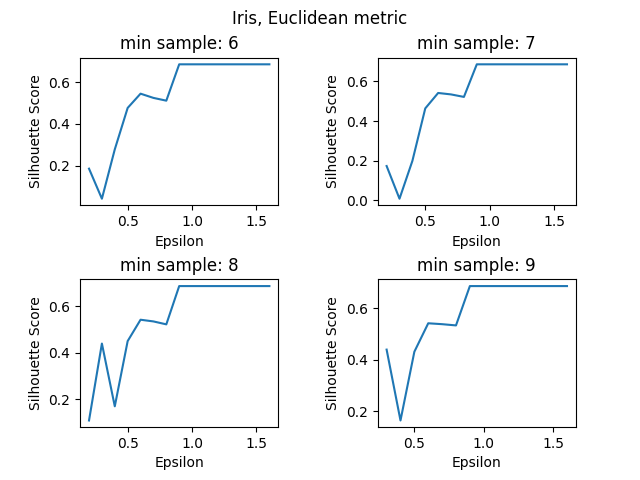
\includegraphics
                    [width=0.9\textwidth,keepaspectratio]
                    {img/db_scan_chart_Iris_eucl1-141824.png}
                    \caption{}
                    \label{db_scan_chart_Iris_eucl1-141824}
                \end{figure}
                \FloatBarrier

            %--------------------------------------------------------------------------------------%

                \begin{figure}[!htbp]
                    \centering
                    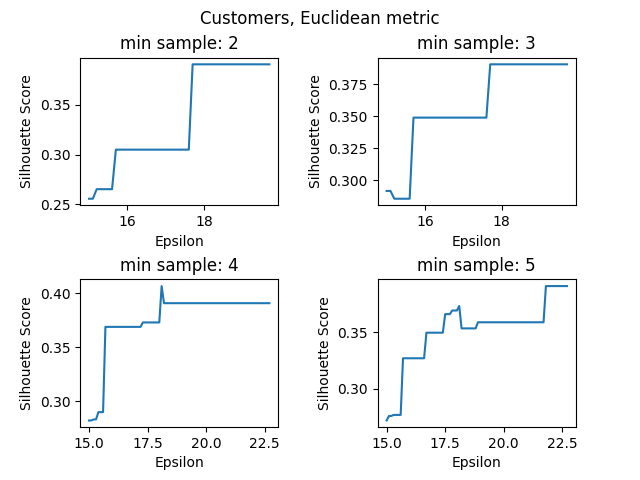
\includegraphics
                    [width=\textwidth,keepaspectratio]
                    {img/db_scan_chart_Customers_eucl0-134449.png}
                    \caption{}
                    \label{db_scan_chart_Customers_eucl0-134449}
                \end{figure}
                \FloatBarrier

                \begin{figure}[!htbp]
                    \centering
                    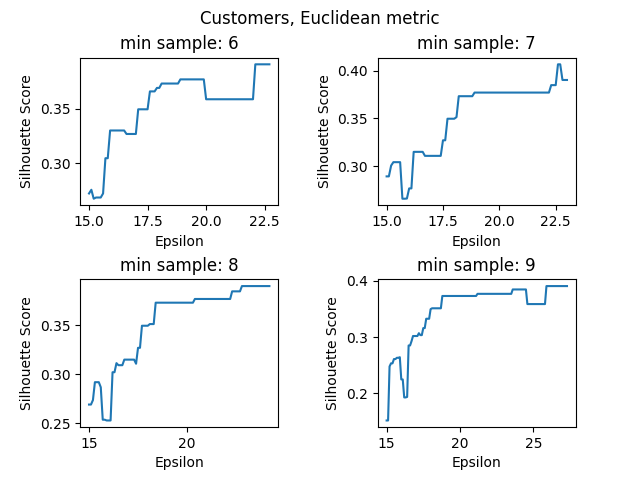
\includegraphics
                    [width=\textwidth,keepaspectratio]
                    {img/db_scan_chart_Customers_eucl1-134449.png}
                    \caption{}
                    \label{db_scan_chart_Customers_eucl1-134449}
                \end{figure}
                \FloatBarrier

            %--------------------------------------------------------------------------------------%

                \begin{figure}[!htbp]
                    \centering
                    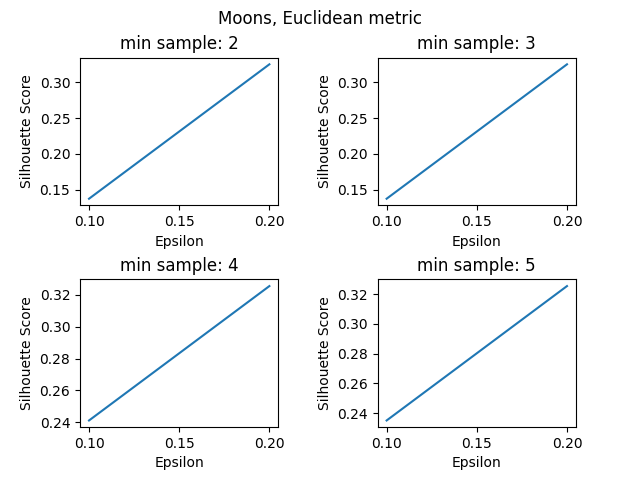
\includegraphics
                    [width=\textwidth,keepaspectratio]
                    {img/db_scan_chart_Moons_eucl0-141858.png}
                    \caption{}
                    \label{db_scan_chart_Moons_eucl0-141858}
                \end{figure}
                \FloatBarrier

                \begin{figure}[!htbp]
                    \centering
                    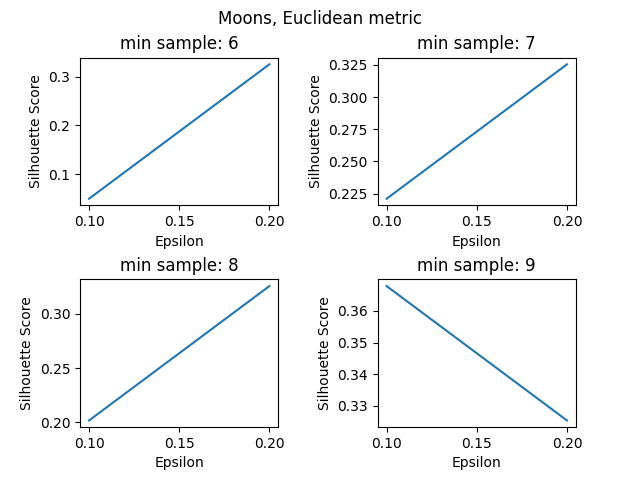
\includegraphics
                    [width=\textwidth,keepaspectratio]
                    {img/db_scan_chart_Moons_eucl1-141858.png}
                    \caption{}
                    \label{db_scan_chart_Moons_eucl1-141858}
                \end{figure}
                \FloatBarrier


                \begin{table}[!htbp]
                    \begin{minipage}{.24\textwidth}
                        \centering
                        \begin{tabular}{|c|c|}
                            \hline
                            Eps & Silh \\ \hline
                            0.1 & 0.1371 \\ \hline
                            0.2 & 0.3254 \\ \hline
                        \end{tabular}
                        \caption
                        [Moons, min samples: 2]
                        {Moons, min samples: 2}
                        \label{db_scan_table_Moons_eucl_min_sample2}
                    \end{minipage}
                    \hfill
                    \begin{minipage}{.24\textwidth}
                        \centering
                        \begin{tabular}{|c|c|}
                            \hline
                            Eps & Silh \\ \hline
                            0.1 & 0.1371 \\ \hline
                            0.2 & 0.3254 \\ \hline
                        \end{tabular}
                        \caption
                        [Moons, min samples: 3]
                        {Moons, min samples: 3}
                        \label{db_scan_table_Moons_eucl_min_sample3}
                    \end{minipage}
                    \hfill
                    \begin{minipage}{.24\textwidth}
                        \centering
                        \begin{tabular}{|c|c|}
                            \hline
                            Eps & Silh \\ \hline
                            0.1 & 0.2412 \\ \hline
                            0.2 & 0.3254 \\ \hline
                        \end{tabular}
                        \caption
                        [Moons, min samples: 4]
                        {Moons, min samples: 4}
                        \label{db_scan_table_Moons_eucl_min_sample4}
                    \end{minipage}
                    \hfill
                    \begin{minipage}{.24\textwidth}
                        \centering
                        \begin{tabular}{|c|c|}
                            \hline
                            Eps & Silh \\ \hline
                            0.1 & 0.235 \\ \hline
                            0.2 & 0.3254 \\ \hline
                        \end{tabular}
                        \caption
                        [Moons, min samples: 5]
                        {Moons, min samples: 5}
                        \label{db_scan_table_Moons_eucl_min_sample5}
                    \end{minipage}
                \end{table}
                \FloatBarrier


                \begin{table}[!htbp]
                    \begin{minipage}{.24\textwidth}
                        \centering
                        \begin{tabular}{|c|c|}
                            \hline
                            Eps & Silh \\ \hline
                            0.1 & 0.0492 \\ \hline
                            0.2 & 0.3254 \\ \hline
                        \end{tabular}
                        \caption
                        [Moons, min samples: 6]
                        {Moons, min samples: 6}
                        \label{db_scan_table_Moons_eucl_min_sample6}
                    \end{minipage}
                    \hfill
                    \begin{minipage}{.24\textwidth}
                        \centering
                        \begin{tabular}{|c|c|}
                            \hline
                            Eps & Silh \\ \hline
                            0.1 & 0.2211 \\ \hline
                            0.2 & 0.3254 \\ \hline
                        \end{tabular}
                        \caption
                        [Moons, min samples: 7]
                        {Moons, min samples: 7}
                        \label{db_scan_table_Moons_eucl_min_sample7}
                    \end{minipage}
                    \hfill
                    \begin{minipage}{.24\textwidth}
                        \centering
                        \begin{tabular}{|c|c|}
                            \hline
                            Eps & Silh \\ \hline
                            0.1 & 0.2018 \\ \hline
                            0.2 & 0.3254 \\ \hline
                        \end{tabular}
                        \caption
                        [Moons, min samples: 8]
                        {Moons, min samples: 8}
                        \label{db_scan_table_Moons_eucl_min_sample8}
                    \end{minipage}
                    \hfill
                    \begin{minipage}{.24\textwidth}
                        \centering
                        \begin{tabular}{|c|c|}
                            \hline
                            Eps & Silh \\ \hline
                            0.1 & 0.3678 \\ \hline
                            0.2 & 0.3254 \\ \hline
                        \end{tabular}
                        \caption
                        [Moons, min samples: 9]{Moons, min samples: 9}
                        \label{db_scan_table_Moons_eucl_min_sample9}
                    \end{minipage}
                \end{table}
                \FloatBarrier

            }

            \subsubsection{Metryka Manhattan}
            \label{dbscan_manh} {

                \begin{table}[!htbp]
                    \begin{minipage}{.24\textwidth}
                        \centering
                        \begin{tabular}{|c|c|}
                            \hline
                            Eps & Silh \\ \hline
                            0.1 & -0.5147 \\ \hline
                            0.2 & -0.4523 \\ \hline
                            0.3 & -0.2502 \\ \hline
                            0.4 & -0.0944 \\ \hline
                            0.5 & 0.002 \\ \hline
                            0.6 & 0.2219 \\ \hline
                            0.7 & 0.1472 \\ \hline
                            0.8 & 0.372 \\ \hline
                            0.9 & 0.2968 \\ \hline
                            1.0 & 0.4082 \\ \hline
                            1.1 & 0.4082 \\ \hline
                            1.2 & 0.6864 \\ \hline
                            1.3 & 0.6864 \\ \hline
                            1.4 & 0.6864 \\ \hline
                            1.5 & 0.6864 \\ \hline
                            1.6 & 0.6864 \\ \hline
                            1.7 & 0.6864 \\ \hline
                            1.8 & 0.6864 \\ \hline
                            1.9 & 0.6864 \\ \hline
                            2.0 & 0.6864 \\ \hline
                            2.1 & 0.6864 \\ \hline
                            2.2 & 0.6864 \\ \hline
                            2.3 & 0.6864 \\ \hline
                            2.4 & 0.6864 \\ \hline
                            2.5 & 0.6864 \\ \hline
                            2.6 & 0.6864 \\ \hline
                        \end{tabular}
                        \caption
                        [Iris, min samples: 2]
                        {Iris, min samples: 2}
                        \label{db_scan_table_Iris_manh_min_sample2}
                    \end{minipage}
                    \hfill
                    \begin{minipage}{.24\textwidth}
                        \centering
                        \begin{tabular}{|c|c|}
                            \hline
                            Eps & Silh \\ \hline
                            0.1 & 0.0439 \\ \hline
                            0.2 & 0.0758 \\ \hline
                            0.3 & -0.3269 \\ \hline
                            0.4 & -0.069 \\ \hline
                            0.5 & 0.0106 \\ \hline
                            0.6 & 0.294 \\ \hline
                            0.7 & 0.2805 \\ \hline
                            0.8 & 0.3671 \\ \hline
                            0.9 & 0.3491 \\ \hline
                            1.0 & 0.4873 \\ \hline
                            1.1 & 0.4873 \\ \hline
                            1.2 & 0.6864 \\ \hline
                            1.3 & 0.6864 \\ \hline
                            1.4 & 0.6864 \\ \hline
                            1.5 & 0.6864 \\ \hline
                            1.6 & 0.6864 \\ \hline
                            1.7 & 0.6864 \\ \hline
                            1.8 & 0.6864 \\ \hline
                            1.9 & 0.6864 \\ \hline
                            2.0 & 0.6864 \\ \hline
                            2.1 & 0.6864 \\ \hline
                            2.2 & 0.6864 \\ \hline
                            2.3 & 0.6864 \\ \hline
                            2.4 & 0.6864 \\ \hline
                            2.5 & 0.6864 \\ \hline
                            2.6 & 0.6864 \\ \hline
                        \end{tabular}
                        \caption
                        [Iris, min samples: 3]
                        {Iris, min samples: 3}
                        \label{db_scan_table_Iris_manh_min_sample3}
                    \end{minipage}
                    \hfill
                    \begin{minipage}{.24\textwidth}
                        \centering
                        \begin{tabular}{|c|c|}
                            \hline
                            Eps & Silh \\ \hline
                            0.3 & 0.2341 \\ \hline
                            0.4 & -0.133 \\ \hline
                            0.5 & 0.0696 \\ \hline
                            0.6 & 0.3107 \\ \hline
                            0.7 & 0.3698 \\ \hline
                            0.8 & 0.4001 \\ \hline
                            0.9 & 0.3872 \\ \hline
                            1.0 & 0.5028 \\ \hline
                            1.1 & 0.4873 \\ \hline
                            1.2 & 0.4881 \\ \hline
                            1.3 & 0.6864 \\ \hline
                            1.4 & 0.6864 \\ \hline
                            1.5 & 0.6864 \\ \hline
                            1.6 & 0.6864 \\ \hline
                            1.7 & 0.6864 \\ \hline
                            1.8 & 0.6864 \\ \hline
                            1.9 & 0.6864 \\ \hline
                            2.0 & 0.6864 \\ \hline
                            2.1 & 0.6864 \\ \hline
                            2.2 & 0.6864 \\ \hline
                            2.3 & 0.6864 \\ \hline
                            2.4 & 0.6864 \\ \hline
                            2.5 & 0.6864 \\ \hline
                            2.6 & 0.6864 \\ \hline
                        \end{tabular}
                        \caption
                        [Iris, min samples: 4]
                        {Iris, min samples: 4}
                        \label{db_scan_table_Iris_manh_min_sample4}
                    \end{minipage}
                    \hfill
                    \begin{minipage}{.24\textwidth}
                        \centering
                        \begin{tabular}{|c|c|}
                            \hline
                            Eps & Silh \\ \hline
                            0.3 & 0.1762 \\ \hline
                            0.4 & -0.0344 \\ \hline
                            0.5 & -0.009 \\ \hline
                            0.6 & 0.2596 \\ \hline
                            0.7 & 0.4545 \\ \hline
                            0.8 & 0.4994 \\ \hline
                            0.9 & 0.5216 \\ \hline
                            1.0 & 0.5117 \\ \hline
                            1.1 & 0.4873 \\ \hline
                            1.2 & 0.4881 \\ \hline
                            1.3 & 0.4881 \\ \hline
                            1.4 & 0.6864 \\ \hline
                            1.5 & 0.6864 \\ \hline
                            1.6 & 0.6864 \\ \hline
                            1.7 & 0.6864 \\ \hline
                            1.8 & 0.6864 \\ \hline
                            1.9 & 0.6864 \\ \hline
                            2.0 & 0.6864 \\ \hline
                            2.1 & 0.6864 \\ \hline
                            2.2 & 0.6864 \\ \hline
                            2.3 & 0.6864 \\ \hline
                            2.4 & 0.6864 \\ \hline
                            2.5 & 0.6864 \\ \hline
                            2.6 & 0.6864 \\ \hline
                        \end{tabular}
                        \caption
                        [Iris, min samples: 5]
                        {Iris, min samples: 5}
                        \label{db_scan_table_Iris_manh_min_sample5}
                    \end{minipage}
                \end{table}
                \FloatBarrier

                \begin{figure}[!htbp]
                    \centering
                    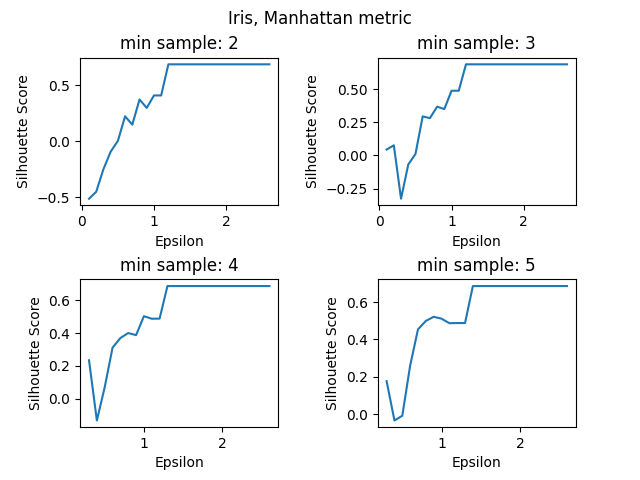
\includegraphics
                    [width=\textwidth,keepaspectratio]
                    {img/db_scan_chart_Iris_manh0-121524.png}
                    \caption{}
                    \label{db_scan_chart_Iris_manh0-121524}
                \end{figure}
                \FloatBarrier


                \begin{table}[!htbp]
                    \begin{minipage}{.24\textwidth}
                        \centering
                        \begin{tabular}{|c|c|}
                            \hline
                            Eps & Silh \\ \hline
                            0.3 & 0.1232 \\ \hline
                            0.4 & -0.1083 \\ \hline
                            0.5 & -0.0258 \\ \hline
                            0.6 & 0.1805 \\ \hline
                            0.7 & 0.4414 \\ \hline
                            0.8 & 0.498 \\ \hline
                            0.9 & 0.5211 \\ \hline
                            1.0 & 0.5298 \\ \hline
                            1.1 & 0.5097 \\ \hline
                            1.2 & 0.4881 \\ \hline
                            1.3 & 0.4881 \\ \hline
                            1.4 & 0.6864 \\ \hline
                            1.5 & 0.6864 \\ \hline
                            1.6 & 0.6864 \\ \hline
                            1.7 & 0.6864 \\ \hline
                            1.8 & 0.6864 \\ \hline
                            1.9 & 0.6864 \\ \hline
                            2.0 & 0.6864 \\ \hline
                            2.1 & 0.6864 \\ \hline
                            2.2 & 0.6864 \\ \hline
                            2.3 & 0.6864 \\ \hline
                            2.4 & 0.6864 \\ \hline
                            2.5 & 0.6864 \\ \hline
                            2.6 & 0.6864 \\ \hline
                        \end{tabular}
                        \caption
                        [Iris, min samples: 6]
                        {Iris, min samples: 6}
                        \label{db_scan_table_Iris_manh_min_sample6}
                    \end{minipage}
                    \hfill
                    \begin{minipage}{.24\textwidth}
                        \centering
                        \begin{tabular}{|c|c|}
                            \hline
                            Eps & Silh \\ \hline
                            0.3 & 0.1232 \\ \hline
                            0.4 & 0.3256 \\ \hline
                            0.5 & 0.1163 \\ \hline
                            0.6 & 0.124 \\ \hline
                            0.7 & 0.4152 \\ \hline
                            0.8 & 0.498 \\ \hline
                            0.9 & 0.5211 \\ \hline
                            1.0 & 0.533 \\ \hline
                            1.1 & 0.5193 \\ \hline
                            1.2 & 0.5446 \\ \hline
                            1.3 & 0.4881 \\ \hline
                            1.4 & 0.6864 \\ \hline
                            1.5 & 0.6864 \\ \hline
                            1.6 & 0.6864 \\ \hline
                            1.7 & 0.6864 \\ \hline
                            1.8 & 0.6864 \\ \hline
                            1.9 & 0.6864 \\ \hline
                            2.0 & 0.6864 \\ \hline
                            2.1 & 0.6864 \\ \hline
                            2.2 & 0.6864 \\ \hline
                            2.3 & 0.6864 \\ \hline
                            2.4 & 0.6864 \\ \hline
                            2.5 & 0.6864 \\ \hline
                            2.6 & 0.6864 \\ \hline
                        \end{tabular}
                        \caption
                        [Iris, min samples: 7]
                        {Iris, min samples: 7}
                        \label{db_scan_table_Iris_manh_min_sample7}
                    \end{minipage}
                    \hfill
                    \begin{minipage}{.24\textwidth}
                        \centering
                        \begin{tabular}{|c|c|}
                            \hline
                            Eps & Silh \\ \hline
                            0.3 & 0.1232 \\ \hline
                            0.4 & 0.1917 \\ \hline
                            0.5 & 0.0599 \\ \hline
                            0.6 & 0.2044 \\ \hline
                            0.7 & 0.3005 \\ \hline
                            0.8 & 0.4862 \\ \hline
                            0.9 & 0.5211 \\ \hline
                            1.0 & 0.533 \\ \hline
                            1.1 & 0.5193 \\ \hline
                            1.2 & 0.5446 \\ \hline
                            1.3 & 0.5446 \\ \hline
                            1.4 & 0.6864 \\ \hline
                            1.5 & 0.6864 \\ \hline
                            1.6 & 0.6864 \\ \hline
                            1.7 & 0.6864 \\ \hline
                            1.8 & 0.6864 \\ \hline
                            1.9 & 0.6864 \\ \hline
                            2.0 & 0.6864 \\ \hline
                            2.1 & 0.6864 \\ \hline
                            2.2 & 0.6864 \\ \hline
                            2.3 & 0.6864 \\ \hline
                            2.4 & 0.6864 \\ \hline
                            2.5 & 0.6864 \\ \hline
                            2.6 & 0.6864 \\ \hline
                        \end{tabular}
                        \caption
                        [Iris, min samples: 8]
                        {Iris, min samples: 8}
                        \label{db_scan_table_Iris_manh_min_sample8}
                    \end{minipage}
                    \hfill
                    \begin{minipage}{.24\textwidth}
                        \centering
                        \begin{tabular}{|c|c|}
                            \hline
                            Eps & Silh \\ \hline
                            0.3 & 0.1232 \\ \hline
                            0.4 & 0.1897 \\ \hline
                            0.5 & 0.0286 \\ \hline
                            0.6 & 0.1882 \\ \hline
                            0.7 & 0.1841 \\ \hline
                            0.8 & 0.4744 \\ \hline
                            0.9 & 0.5211 \\ \hline
                            1.0 & 0.533 \\ \hline
                            1.1 & 0.5295 \\ \hline
                            1.2 & 0.5471 \\ \hline
                            1.3 & 0.5474 \\ \hline
                            1.4 & 0.6864 \\ \hline
                            1.5 & 0.6864 \\ \hline
                            1.6 & 0.6864 \\ \hline
                            1.7 & 0.6864 \\ \hline
                            1.8 & 0.6864 \\ \hline
                            1.9 & 0.6864 \\ \hline
                            2.0 & 0.6864 \\ \hline
                            2.1 & 0.6864 \\ \hline
                            2.2 & 0.6864 \\ \hline
                            2.3 & 0.6864 \\ \hline
                            2.4 & 0.6864 \\ \hline
                            2.5 & 0.6864 \\ \hline
                            2.6 & 0.6864 \\ \hline
                        \end{tabular}
                        \caption
                        [Iris, min samples: 9]
                        {Iris, min samples: 9}
                        \label{db_scan_table_Iris_manh_min_sample9}
                    \end{minipage}
                \end{table}
                \FloatBarrier

                \begin{figure}[!htbp]
                    \centering
                    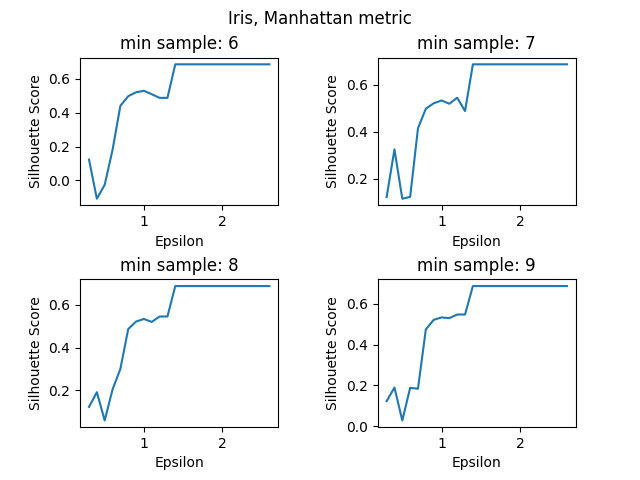
\includegraphics
                    [width=\textwidth,keepaspectratio]
                    {img/db_scan_chart_Iris_manh1-121525.png}
                    \caption{}
                    \label{db_scan_chart_Iris_manh1-121525}
                \end{figure}
                \FloatBarrier


            %--------------------------------------------------------------------------------------%

                \begin{figure}[!htbp]
                    \centering
                    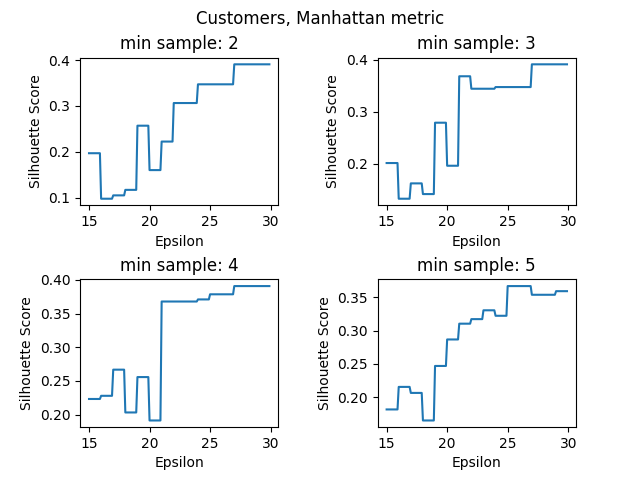
\includegraphics
                    [width=\textwidth,keepaspectratio]
                    {img/db_scan_chart_Customers_manh0-134459.png}
                    \caption{}
                    \label{db_scan_chart_Customers_manh0-134459}
                \end{figure}
                \FloatBarrier

                \begin{figure}[!htbp]
                    \centering
                    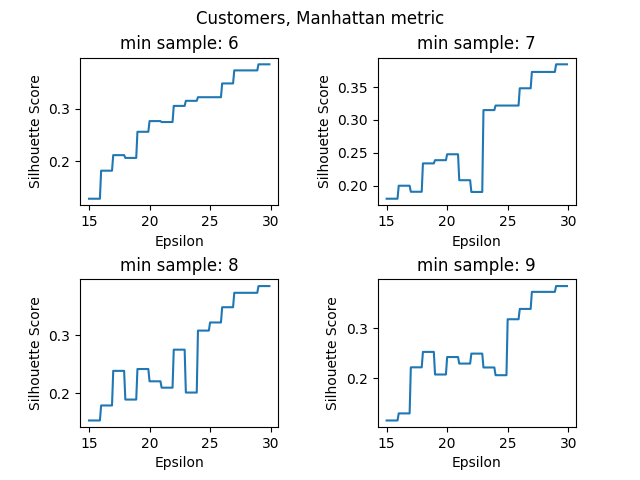
\includegraphics
                    [width=\textwidth,keepaspectratio]
                    {img/db_scan_chart_Customers_manh1-134459.png}
                    \caption{}
                    \label{db_scan_chart_Customers_manh1-134459}
                \end{figure}
                \FloatBarrier


            %--------------------------------------------------------------------------------------%

                \begin{figure}[!htbp]
                    \centering
                    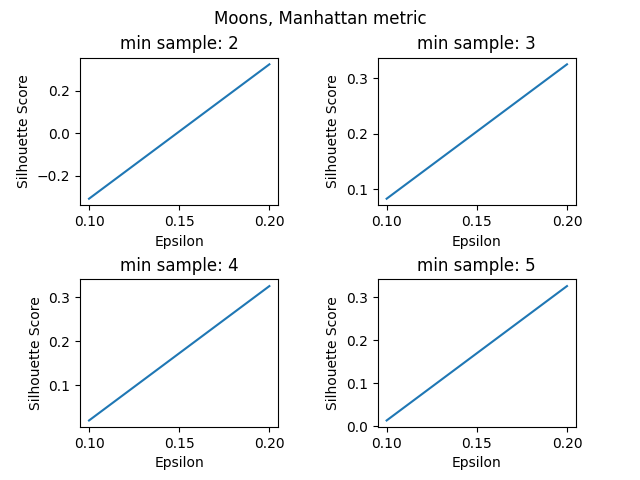
\includegraphics
                    [width=\textwidth,keepaspectratio]
                    {img/db_scan_chart_Moons_manh0-121542.png}
                    \caption{}
                    \label{db_scan_chart_Moons_manh0-121542}
                \end{figure}
                \FloatBarrier

                \begin{figure}[!htbp]
                    \centering
                    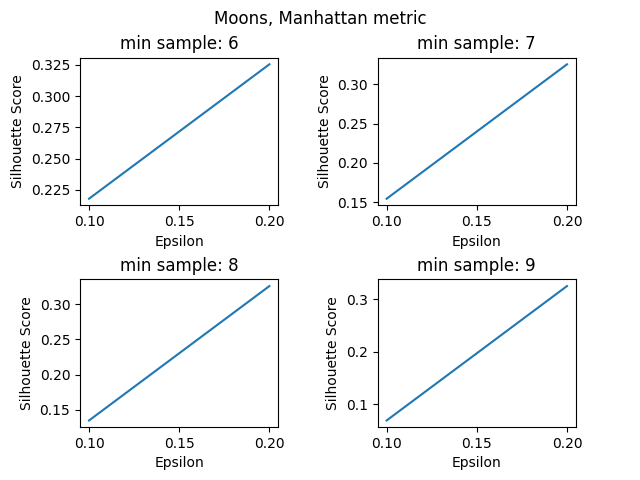
\includegraphics
                    [width=\textwidth,keepaspectratio]
                    {img/db_scan_chart_Moons_manh1-121543.png}
                    \caption{}
                    \label{db_scan_chart_Moons_manh1-121543}
                \end{figure}
                \FloatBarrier

                \begin{table}[!htbp]
                    \begin{minipage}{.24\textwidth}
                        \centering
                        \begin{tabular}{|c|c|}
                            \hline
                            Eps & Silh \\ \hline
                            0.1 & -0.3083 \\ \hline
                            0.2 & 0.3254 \\ \hline
                        \end{tabular}
                        \caption
                        [Moons, min samples: 2]
                        {Moons, min samples: 2}
                        \label{db_scan_table_Moons_manh_min_sample2}
                    \end{minipage}
                    \hfill
                    \begin{minipage}{.24\textwidth}
                        \centering
                        \begin{tabular}{|c|c|}
                            \hline
                            Eps & Silh \\ \hline
                            0.1 & 0.083 \\ \hline
                            0.2 & 0.3254 \\ \hline
                        \end{tabular}
                        \caption
                        [Moons, min samples: 3]
                        {Moons, min samples: 3}
                        \label{db_scan_table_Moons_manh_min_sample3}
                    \end{minipage}
                    \hfill
                    \begin{minipage}{.24\textwidth}
                        \centering
                        \begin{tabular}{|c|c|}
                            \hline
                            Eps & Silh \\ \hline
                            0.1 & 0.0192 \\ \hline
                            0.2 & 0.3254 \\ \hline
                        \end{tabular}
                        \caption
                        [Moons, min samples: 4]
                        {Moons, min samples: 4}
                        \label{db_scan_table_Moons_manh_min_sample4}
                    \end{minipage}
                    \hfill
                    \begin{minipage}{.24\textwidth}
                        \centering
                        \begin{tabular}{|c|c|}
                            \hline
                            Eps & Silh \\ \hline
                            0.1 & 0.0136 \\ \hline
                            0.2 & 0.3254 \\ \hline
                        \end{tabular}
                        \caption
                        [Moons, min samples: 5]
                        {Moons, min samples: 5}
                        \label{db_scan_table_Moons_manh_min_sample5}
                    \end{minipage}
                \end{table}
                \FloatBarrier


                \begin{table}[!htbp]
                    \begin{minipage}{.24\textwidth}
                        \centering
                        \begin{tabular}{|c|c|}
                            \hline
                            Eps & Silh \\ \hline
                            0.1 & 0.218 \\ \hline
                            0.2 & 0.3254 \\ \hline
                        \end{tabular}
                        \caption
                        [Moons, min samples: 6]
                        {Moons, min samples: 6}
                        \label{db_scan_table_Moons_manh_min_sample6}
                    \end{minipage}
                    \hfill
                    \begin{minipage}{.24\textwidth}
                        \centering
                        \begin{tabular}{|c|c|}
                            \hline
                            Eps & Silh \\ \hline
                            0.1 & 0.1543 \\ \hline
                            0.2 & 0.3254 \\ \hline
                        \end{tabular}
                        \caption
                        [Moons, min samples: 7]
                        {Moons, min samples: 7}
                        \label{db_scan_table_Moons_manh_min_sample7}
                    \end{minipage}
                    \hfill
                    \begin{minipage}{.24\textwidth}
                        \centering
                        \begin{tabular}{|c|c|}
                            \hline
                            Eps & Silh \\ \hline
                            0.1 & 0.135 \\ \hline
                            0.2 & 0.3254 \\ \hline
                        \end{tabular}
                        \caption
                        [Moons, min samples: 8]
                        {Moons, min samples: 8}
                        \label{db_scan_table_Moons_manh_min_sample8}
                    \end{minipage}
                    \hfill
                    \begin{minipage}{.24\textwidth}
                        \centering
                        \begin{tabular}{|c|c|}
                            \hline
                            Eps & Silh \\ \hline
                            0.1 & 0.0688 \\ \hline
                            0.2 & 0.3254 \\ \hline
                        \end{tabular}
                        \caption
                        [Moons, min samples: 9]
                        {Moons, min samples: 9}
                        \label{db_scan_table_Moons_manh_min_sample9}
                    \end{minipage}
                \end{table}
                \FloatBarrier


            }

        }

    }

    \section{Dyskusja}
    \label{summary} {

        \subsection{Algorytm k-średnich}
        \label{summary_1} {
            Analizując wartości współczynnika zarysu dla zbioru \cite{dataset_iris},
            dzięki tabeli \ref{kmeans_table_clusters_Iris} oraz wizualizacji tych
            danych zawartych na wykresie \ref{kmeans_chart_Iris_173201} można
            wywnioskować, że optymalną liczbą klastrów jest liczba 2, natomiast
            wartości współczynnika zarysu dla liczby klastrów większej od 5 drastycznie
            spadają, przez co należy uznać je jako nieodpowiednie dla tego zbioru.
            Natomiast badanie wpływu wartości maksymalnej liczby iteracji wskazało, że
            największy wpływ na wartość współczynnika zarysu ma liczba z przedziału
            [1e9; 1e11] dla liczby klastrów równej 19 lub 25. Niestety dla pozostałych
            wartości liczby klastrów nie zauważono żadnej wartości maksymalnej liczby
            iteracji, którą należałoby dokładniej zbadać - nie udało się ustalić rzędu
            wielkości tego parametru, który mógłby mieć wpływ na końcowy wynik.

            Analizując wartości współczynnika zarysu dla zbioru
            \cite{dataset_customers}, dzięki tabeli
            \ref{kmeans_table_clusters_Customers} oraz wizualizacji tych danych
            zawartych na wykresie \ref{kmeans_chart_Customers_173204} można
            wywnioskować, że optymalną liczbą klastrów jest liczba z przedziału [5; 8],
            gdyż dla tego przedziału współczynnik zarysu osiągał najwyższe wartości.
            Warto zauważyć, że dla liczby klastrów równej 29, dla tego zbioru danych,
            widać delikatny wzrost dokładności, dlatego zasadne może okazać się
            wykorzystanie go przy odpowiedniej manipulacji innymi parametrami.
            Natomiast badanie wpływu wartości maksymalnej liczby iteracji wskazało, że
            największy wpływ na wartość współczynnika zarysu ma liczba z przedziału
            [1e6; 1e11] dla liczby klastrów równej 19 lub 25. Warty zauważenia jet
            fakt, że dal liczby klastrów równej 8, między wartościami 1e10 a 1e11
            zaobserwowano wzrost wartości współczynnika zarysu, co może świadczyć o
            tym, że dobranie maksymalnej liczby iteracji o podobnej wartości do
            wymienionych może skutkować wzrostem wartości współczynnika. Niestety dla
            pozostałych wartości liczby klastrów nie zauważono żadnej wartości
            maksymalnej liczby iteracji, którą należałoby dokładniej zbadać - nie udało
            się ustalić rzędu wielkości tego parametru, który mógłby mieć wpływ na
            końcowy wynik.

            Analizując wartości współczynnika zarysu dla zbioru \cite{dataset_moons},
            dzięki tabeli \ref{kmeans_table_clusters_Moons} oraz wizualizacji tych
            danych zawartych na wykresie \ref{kmeans_chart_Moons_173215} można
            wywnioskować, że optymalną liczbą klastrów jest liczba naturalna z przedziału [6;
            10], gdyż dla tego przedziału współczynnik zarysu osiągał najwyższe
            wartości. Warto zauważyć, że dla liczby klastrów większej niż 25, dla tego
            zbioru danych, widać delikatny wzrost dokładności, dlatego zasadne może
            okazać się wykorzystanie tej wartości przy odpowiedniej manipulacji innymi
            parametrami. Natomiast badanie wpływu wartości maksymalnej liczby iteracji
            wskazało, że największy wpływ na wartość współczynnika zarysu ma liczba z
            przedziału [1e7; 1e101] dla liczby klastrów równej 25. Niestety dla
            pozostałych wartości liczby klastrów nie zauważono żadnej wartości
            maksymalnej liczby iteracji, którą należałoby dokładniej zbadać - nie udało
            się ustalić rzędu wielkości tego parametru, który mógłby mieć wpływ na
            końcowy wynik.
            
        
        }

        \subsection{Algorytm aglomeracyjny}
        \label{summary_2} {
            Rysunki \ref{fig:agglomerative_iris}, \ref{fig:agglomerative_customers}
            oraz \ref{fig:agglomerative_moons} przedstawiają wyniki klasteryzacji
            trzech zbiorów danych, z wykorzystaniem algorytmu aglomeracyjnego. Podobnie
            jak w przypadku pozostałych metod grupowania, jako miarę jakości podziału
            danych przyjęto \emph{współczynnik zarysu}. Każdy z wymienionych rysunków
            zawiera cztery wykresy, dla czterech różnych metod łączenia (ang.
            \emph{linkage}). Zmienną zależną na wykresach jest wartość współczynnika
            zarysu a niezależną - liczba klastrów, na które został podzielony zbiór
            danych. Dodatkowo trzy z czterech wykresów zawierają po dwie krzywe, każda
            związana z inną metryką wykorzystaną przez algorytm aglomeracyjny.
            Wyjątkiem jest tutaj metoda łączenia Warda, ponieważ wymaga ona
            wykorzystania metryki euklidesowej, do poprawnego działania. W legendzie
            wykresów zamieszczona została również maksymalna (czyli najlepsza) wartość
            współczynnika zarysu, jaką udało się dla danych parametrów uzyskać. Tak
            więc w sumie zbadana została jakość grupowania danych przez algorytm
            aglomeracyjny w zależności od trzech różnych parametrów:
            \begin{itemize}
                \item liczba klastrów
                \item metoda łączenia
                \item metryka
            \end{itemize}

            Pierwszym zbiorem danych poddanym klasteryzacji jest zbiór ,,Iris Species''
            . Z rysunku \ref{fig:agglomerative_iris} można łatwo wywnioskować, że
            najlepsze wyniki daje podział na 2 klastry, co dla wszystkich metod
            łączenia z wyjątkiem \emph{complete} pozwala osiągnąć wartość współczynnika
            zarysu równą $0.69$. Jest to wartość ,,dobra'', oznacza, że udało się
            zdecydowania podzielić zbiór na odseparowane od siebie grupy, nie oznacza
            to jednak, że jest to podział najlepszy. Wiemy zresztą z góry, że różnych
            gatunków irysów w tym zbiorze są trzy. Mogły wydarzyć się różne rzeczy,
            przykładowo dwie klasy irysów zostały sklejona, lub jedna rozbita na części
            i przyporządkowana do dwóch pozostałych. Warto mieć na uwadze, że zadanie
            klasteryzacji jest o tyle specyficzne, że trudno tak naprawdę ocenić jakość
            podziału danych na grupy, zwłaszcza wtedy, kiedy nie wiadomo ile tych grup
            powinno być. W przypadku wyników związanych z tym zbiorem można, między
            innymi, zwrócić jeszcze uwagę na dwie sprawy. Po pierwsze pojedyncza metoda
            łączenia, dla większej liczby klastrów, osiąga znacznie gorsze wyniki niż
            pozostałem metody - współczynnik zarysu schodzi nawet poniżej zera. To
            pokazuje jej wrażliwość na dane odstające i tendencję do tworzenia mniej
            sferycznych struktur. Po drugie ciekawe są wyniki na drugim wykresie w
            pierwszym rzędzie, gdziem można dostrzec, że dla metryki miejskiej,
            najlepszą wartość współczynnika zarysu daje podział na 3 klastry, co jest
            zgodne z faktycznym podziałem tego zbioru. Można by wysnuć jeszcze wiele
            ciekawszych wniosków, gdyby zastosować dla tego zbioru miary zewnętrzne,
            pozwalające uwzględnić wiedzę o rzeczywistych klasach próbek.

            Na rys. \ref{fig:agglomerative_customers} dzieje się już znacznie więcej,
            niż w przypadku zbioru danych irysów. Widać tutaj wyraźnie, że podział na
            dwie grupy nie jest najlepszym pomysłem. Nie możemy natomiast skonfrontować
            tego spostrzeżenia z faktycznym podziałem danych, gdyż nie jest on znany.
            Stajemy więc przed najbardziej rzeczywistym problemem klasteryzacji,
            rozwiązywanym w ramach tego zadania. Dla metod łączenia ,,complete'' i ,,
            average'' widać, że najlepiej wypada podział danych na 5 grup. W przypadku
            obu tych metod taki podział prowadzi również do tej samej wartości
            współczynnika zarysu, jaką jest $0.44$. Pomijając fakt, że jest to
            najlepsza osiągnięta wartość w tym zadaniu, to w ogóle nie jest to wynik,
            który można uznać za bardzo dobry. Należy jednak pamiętać, że wartość tej
            miary może być zupełnie różna nawet dla dobrych podziałów zbiorów, ale o
            różnej charakterystyce. Warto jeszcze w tym momencie podkreślić, że jest
            dość duże podobieństwo między metodami łączenia ,,complete'' i ,,average'',
            co widać w podobieństwie wykresów drugiego i trzeciego. Trochę inaczej
            zachowuje się metoda łączenia Warda, która pozwala osiągnąć najwyższą
            wartość współczynnika zarysu dla 6 klastrów, jest ona jednak wciąż bardzo
            zbliżona do wspomnianej wcześniej, najlepszej otrzymanej wartości. W tym
            przypadku metoda łączenia ,,single'' nie sprawuje się zbyt dobrze. Jak
            widać nie odpowiada charakterystyce zbioru, gdzie próbki są być może
            pogrupowane w bardziej sferyczne struktury. Na końcu można jeszcze
            wspomnieć, że obie metryki sprawują się podobnie, zwłaszcza w przypadku
            optymalnej liczby klastrów.

            Ostatni zbiór danych jest, w przeciwieństwie do dwóch poprzednich, jedynie
            dwuwymiarowy. Jest też zupełnie sztucznie wygenerowany. Natomiast jego
            kształt, który przypomina dwa nachodzące na siebie półksiężyce, pozwala
            wyciągnąć wiele ciekawych wniosków na temat metody aglomeracyjnej i samego
            współczynnika zarysu. Po pierwsze należy stwierdzić, że zgodnie z wykresami
            najgorzej sprawuje się metoda łączenia ,,single''. Nie jest to jednak
            zgodne z prawdą, gdyż metoda ta jako jedyna, pozwala faktycznie podzielić
            zbiór danych na dwa wspomniane półksiężyce. Grupy te nie mają sferycznego
            kształtu, więc metoda ta nadaje się do nich najlepiej. Niestety
            współczynnik zarysu nie potraktuje takiego podziału jako najlepszy, gdyż
            jest oparty na średnich odległościach między próbkami. Pozostałem metody
            łączenia dają wyniki podobne, to znaczy współczynnik zarysu na poziomie $0.5$,
            czyli ,,rozsądny'', a optymalna liczba klastrów to $7$ lub $8$. Wynik
            taki oznacza stworzenia w ramach obu półksiężyców niewielkich, sferycznych
            grup. Dla takiego podziału współczynnik zarysu jest znacznie większy niż
            dla podziału na rzeczywiste klasy.
        }

        \subsection{Algorytm EM}
        \label{summary_3} {
            Podczas ewaluacji wyników przeprowadzonych eksperymentów pierwszym
            parametrem, który został poddany analizie była liczba klastrów. Na początku
            program został uruchomiony przy stałej wartości maksymalnej liczby iteracji
            (300) dla liczby klastrów przyjmującej wartość od 1 do 20. Na podstawie
            wyników z wstępnego eksperymentu zostało wybranych 5 wartości (4,6,9,15,20)
            przy których zauważono największe ''załamania'' wykresu i które posłużyły
            jako wartości parametru dla kolejnych testów.

            Dla każdego zbioru optymalna liczba skupisk przyjmuje inną wartość, co jest
            związane z samą charakterystyką danych użytych do eksperymentu. Dla zbioru
            Irysów najlepszą wartością klastrów wydaje się być 4, w przypadku Customers
            jest to 6, a dla zbioru danych Moons najlepsze wyniki były osiągane przy 9
            klastrach. Dla każdego zbioru danych zwiększenie liczby klastrów ponad
            wartość optymalną powodowało coraz częstsze występowanie ujemnych wartości
            współczynnika zarysu wśród testowanych konfiguracji maksymalnych iteracji
            oraz macierzy kowariancji. Różnice między wynikami w ramach sąsiednich
            maksymalnych liczb iteracji również wydawały się większe.

            Kolejnym parametrem, który ulegał zmianie podczas przeprowadzonych testów
            algorytmu była liczba maksymalnych iteracji. Maksymalna liczba iteracji
            została dobrana poniekąd wykładniczo, aby możliwa była analiza zachowania
            metody w przypadku zarówno małych, jak i skrajnie dużych wartości. W
            przypadku każdego zbioru danych można zauważyć pewną prawidłowość. Algorytm
            osiągał zadowalające wyniki nawet w przypadku mniejszych wartości
            maksymalnych iteracji (100 - 200) i nie ulegały one poprawie dla wartości
            większych.

            Ostatnim z parametrów wykorzystywanym podczas rozwiązania problem setu był
            rodzaj macierzy kowariancji stosowanej przy metodzie EM. Dostępne były 4
            warianty, z których każdy wpływa na zachowanie algorytmu:
            \begin{itemize}
                \item \textit{full}
                \item \textit{tied}
                \item \textit{diagonal}
                \item \textit{spherical}
            \end{itemize}
            Przypadek dla każdego zestawu danych należy rozpatrywać indywidualnie, gdyż
            dla każdego zbioru optymalną wartość osiągał inny rodzaj wariantu macierzy
            kowariancji.
        }

        \subsection{Algorytm DBSCAN}
        \label{summary_4} {
            W przypadku metryki Euklidesowej dla zbioru \cite{dataset_iris} można
            zauważyć tendencję, że wraz ze wzrostem minimalnej liczby próbek
            (ang. min samples) wartość współczynnika zarysu (ang. Silhouette score)
            wzrasta dla tych samych wartości epsilon z początku zakresu tzn
            od \textit{eps=0.3} do \textit{eps=0.6}. Jest to szczególnie widoczne gdy
            porównamy tabele \ref{db_scan_table_Iris_eucl_min_sample2} oraz
            \ref{db_scan_table_Iris_eucl_min_sample9}. Ciekawą obserwacją jest też to,
            że od wartości \textit{eps=1.0} dla praktycznie wszystkich zbadanych
            wartości \textit{min samples} wartość \textit{Silhouette score}
            to \textit{0.6864}. Co więcej dziwną sprawą jest, że dla praktycznie
            wszystkich wartości \textit{min samples}, zazwyczaj dla drugiej wartości
            \textit{eps} jest dosyć duży spadek wartości współczynnika zarysu,
            natomiast dla kolejnych wartości można zaobserwować wzrost wartości
            współczynnika aż do osiągnięcia wcześniej wspomnianej wartości maksymalnej.
            Co do samych wartości \textit{eps} to to pomimo zastosowanie liczb z
            przedziału od \textit{0.1} do \textit{9.9} z częstotliwością \textit{0.1}
            udało się uzyskać wyniki tylko do wartości \textit{eps=1.6} bez względu na
            wartość \textit{min samples}. Gdy została użyta metryka Manhattan to do
            osiągnięcia maksymalnej wartości współczynnika zarysu wymaga była wyższa
            wartość \textit{eps} natomiast było możliwe wyznaczenie klastrów dla
            większych wartości \textit{eps} tzn. do wartości \textit{2.6} zamiast
            \textit{1.6}.

            W przypadku zbioru \cite{dataset_customers} dla metryki Euklidesowej
            wartość współczynnika zarysu wzrastała wraz z wartością \textit{eps}. Warto
            tutaj wspomnieć o zmianie w wartościach \textit{eps}, które zostały opisane
            w sekcji \ref{intro}.
            W większości przypadków był to wzrost w miarę liniowy. Najlepszy wynik udało
            się uzyskać dla \textit{min samples=7}. Gdy została użyta metryka Manhattan
            to od razu można zauważyć to, że przyrost wartości \textit{Silhouette score}
            jest mniej liniowy i bardziej \textit{'poszarpany i kwadratowy'} co można
            tłumaczyć charakterem działania metryki. Same wyniki są dosyć porównywalne
            natomiast jest tutaj zachowana ta tendencja co dla zbioru \cite{dataset_iris},
            że wymagane są większe wartości \textit{eps} do uzyskania podobnych
            wartości współczynnika.

            Ostatnim użytym zbiorem jest \cite{dataset_moons}, dla metryki Euklidesowej
            bardzo ciekawą sprawą jest to, że bez względu na wartość
            \textit{min sample}, wartość współczynnika zarysu udało się wyliczyć tylko
            dla wartości \textit{eps} równej \textit{0.1} oraz \textit{0.2} oraz dla
            \textit{eps=0.2} wynik jest zawsze taki sam. Jedyne różnice można zauważyć
            dla \textit{eps=0.1} wraz ze wzrostem \textit{min samples} wzrasta wartość
            \textit{Silhouette score}. Jest to wybitnie widoczne \textit{min samples=9}
            gdy wyjątkowo jest wykres funkcji liniowej, która maleje. Jest to
            spowodowane tym, że właśnie tam udało się uzyskać najlepszy grupowanie a
            wartość współczynnika zarysu była równa \textit{0.3678}. Gdy została użyta
            metryka Manhattan to wyniki dla \textit{eps=0.1} wyniki diametralnie się
            pogorszyły, natomiast dla wartości \textit{eps=0.2} uzyskano takie samo
            maksimum jak dla pierwszej metryki.
        }

    }

    \section{Wnioski}
    \label{conclusions} {
        Podsumowując wykonane zadanie wnioskujemy, że:
        \begin{itemize}
            \item W algorytmie aglomeracyjnym nie ma tak dużego znaczenia wybór
            metryki, natomiast metoda łączenia jest decydująca dla poprawnego
            działania algorytmu
            \item Metoda łączenia ,,single'' algorytmu aglomeracyjnego zazwyczaj
            sprawuje się gorzej, jest bardziej podatna na kształt danych i dane
            odstające, ze zwzględu na swój charakter prowadzi zazwyczaj do
            niższych wartości współczynnika zarysu, pozostałe metody łączenia
            sprawują się podobnie i prowadzą do podobnych podziałów o sferycznym
            kształcie
            \item Sam współczynnik zarysu nie wystarczy aby dobrze ocenić jakość
            klasteryzacji, jest on bardzo zależny od charakterystyki zbioru danych
            \item Dla metody \textit{k-średnich} najważniejszym parametrem jest liczba
            klastrów, która ma największy wpływ na wartość współczynnika zarysu.
            Maksymalna liczba iteracji ma drugorzędne znaczenie, jednakże może ona
            wpłynąć korzystnie na wartość współczynnika zarysu, zwykle jest to
            zaobserwowane dla dużych wartości liczby iteracji, efekt ten jest lepiej
            widoczny dla badania, w którym wykorzystana została większa liczba klastrów.
            \item Dla metody \textit{EM} wybór liczby klastrów ma kluczowe znaczenie dla
            uzyskiwanych wartości współczynnika zarysu. Maksymalna liczba iteracji ma
            natomiast znikomy wpływ na otrzymane wyniki, jednak tak jak w przypadku
            algorytmu k-średnich może one wpłynąć pozytywnie na wartość współczynnika zarysu
            \item Dla metody \textit{EM} optymalne konfiguracje różnią się między
            wybranymi zbiorami danych, dlatego ważne jest dobranie ich indywidualnie dla każdego zestawu danych
            \item Dla metody \textit{DBSCAN} wybór metryki nie wpływa znacząco na
            wyniki natomiast dla metryki Manhattan po prostu potrzebne są większe wartości
            parametru \textit{eps}
            \item Dla metody \textit{DBSCAN} i wybranych zbiorów warto stosować większe
            wartości parametru \textit{min samples}. Samo znajdowanie wartości warto
            przeprowadzać dla danego zbioru gdyż pominiecie tego kroku może pogorszyć
            wyniki

        \end{itemize}
    }

    \begin{thebibliography}{0}
        \bibitem{dataset_iris}{https://www.kaggle.com/uciml/iris}
        \bibitem{dataset_customers}
        {https://www.kaggle.com/vjchoudhary7/customer-segmentation-tutorial-in-python}
        \bibitem{dataset_moons}
        {https://scikit-learn.org/stable/modules/generated/sklearn.datasets.make\_moons.html}

    \end{thebibliography}

\end{document}
